\documentclass[11pt, a4paper]{article}

\usepackage{graphicx}
\usepackage{url}
\usepackage{appendix}
\usepackage{comp520}
\usepackage{pseudocode}

\usepackage[hmargin=2cm,vmargin=2.5cm]{geometry}

%\addtolength{\oddsidemargin}{-.875in}
%\addtolength{\evensidemargin}{-.875in}
%\addtolength{\textwidth}{1.75in}
\linespread{1.5}

\begin{document}
\innertitle{Joel Oughton}{Improved Network Map Display}
\date{26/10/2011}

%\maketitle
\tableofcontents

\newpage

\abs{
  % Adjust my old abstract to reflect overall project state.
}

\section{Introduction}
\label{sec:introduction}
  % Motivation for my project
  % List the achievements (refer to sections)
  %
  %
  % Introduce my project:
  %   > Start with overview of project
  %     * improve introduction from interim report?
  %   > Motivate your project - topic is important and worth reading
  %     and something new to the field
  %   > What is my research question?
  %   > How did I solve it?
  %   > What sort of results will the paper present? 

  % what is the general topic?
  %   - HTML 5 technologies
  %   - modern computer network map display
  %   - what is a network map

Computer network maps are an effective way of visualising complex network
systems. Network maps consist of nodes and edges, where nodes represent devices
and edges show the physical or logical relationship between them. The
positioning of nodes throughout a map, displays the topology of the network that
it is visualising. It is important to get the positioning right because the maps
may be used to gain insight into the shape and structure of network devices.
Automatic layout algorithms may be used to attempt a good layout or users may
want to define static positions for nodes when there is already some idea about
the underlying topology. Also, various users of a network map may need to view
it from different perspectives depending on their roll. For example, a support
desk worker may just need to see whether or not very general areas of the
network are functional, where as a network engineer may need to see a specific
area with a lot of detail.

In network maps, the edges connecting nodes indicate a relationship between two
devices. Networks often monitor and store performance metrics of a link that can
be directly related to a single edge. It is therefore, possible to visualise the
metrics as part of the edge graphics or to include them through user
interaction. This idea assists with two uses of network maps: monitoring and
dimensioning. Network maps can be used to monitor the health of the devices and
links, and visually indicate the user when a problem is detected. With an
effective layout in place, areas of the network that are affected by the problem
can be easily identified and passed on to engineers to look into. Dimensioning
in networks is finding the minimum capacity of a link to service the peak
capacity \cite{Girard_1990}. Network maps which show bandwidth usage on links
effectively can assist network engineers at determining what the peak capacity
of links are and whether there is more bandwidth available that can be sold to
customers.

In this project, techniques and technologies are explored with the goal of
producing an improved network map display over existing implementations.
NetMapJs, a web based network map visualisation application, was designed and
developed as part of this project to present the ideas discussed in this report.
There are some notable weaknesses of existing network maps that this project
aims to address:

\begin{itemize}
  \item Lack of interactivity
  \item Scalability issues with large networks
  \item Specialised software requirements
  \item Limited visual display of quantitative information
\end{itemize}

  % problems with current network maps (Motivation):
  %   > Net very dynamic or interactive, often just static images
  %   > Lack of portability
  %   > Don't scale well to large networks
  %   > Don't consider layers???
  %
  % Design goals
  %   > web based
  %   > Scalable
  %   > Interactive 
  %   > Mutli layered???
 
Network maps often generate static images that provide little or no user
interaction. This project looks into the use of zooming, panning and other
interactive navigation functionality to give users more control over the
information space. A user-friendly event system encourages developers to make
use of user input. Clicking or hovering over nodes and edges for example, calls
event functions that can be customised to add to the visual display without
needing an understanding about how the internals of NetMapJs works. Existing
tools also usually do not scale well for large networks, as views become
overwhelming and overlapping edges obscure parts of the network. This project
considers the use of hierarchy to reduce the overall complexity of maps by
grouping sub networks together. The idea of groups coupled with semantic zooming
enables detail to be abstracted until the user indicates that they are
interested in a more specific area of the network.

Current computer network visualisation tools in the network industry do not take
full advantage of the latest web technologies. Visualisations built and
presented using HTML5 technologies in general are becoming more popular because
the information can be presented in a web browser. This avoids the need to
develop, maintain and install specialised software for multiple systems. Web
browsers are ubiquitous so views can be shared and discussed between users.
Mobile devices also come with browsers which give viewers instant portability.
This project focusses on taking advantage of these technologies in order to
produce a highly interactive computer network map that is easily accessible.

The performance of links between devices in a network coupled with an idea of
topology is useful for capacity management and monitoring. A link may not be
using all of its available bandwidth and so there would be a possibility of
adding additional clients. The opposite is also useful; an indication of high
bandwidth utilisation lets administrators know that more links or load balancing
may be beneficial to their clients. Existing network map implementations
sometimes attempt to display this information in edges or by other means. This
is most commonly either the width line or a set of colours. However, the use of
colour to is one of the least useful ways to display quantitative variables
\cite{Spence_2007}. In this project, a new way of displaying quantitative data
within edges that uses edge width, length, orientation and colouring is
presented and implemented in NetMapJs with good results.

  % The achievements and section breakdowns
  %

The datasets used in this project for testing NetMapJs were sourced from two
real and currently operational networks, Rural Link and KAREN. Both networks
have mapping tools currently in place. A brief comparison of these tools with
NetMapJs are included in this report. In the evaluation section, network
engineers from within Rural Link and KAREN are also asked to compare the tools
and provide feedback. 

This report is divided into the following sections. Section
\ref{sec:related-work} gives the necessary background information used for the
rest of the report. The datasets are described in detail and the technologies
and libraries used in this project are listed. The visual design considerations
are described in Section \ref{sec:visual-design}. Each of the design aspects are
motivated, justified and an example from NetMapJs is given. The technical
details about how the visual design was implemented are found in Section
\ref{sec:implementation}. In Section \ref{sec:evaluation}, the results of
evaluation by network engineers are discussed. Finally, conclusions are drawn
and some possible directions of future work are mentioned in Section
\ref{sec:conclusion}.

\newpage

\section{Related Work}
\label{sec:related-work}
  % ** General Related Work Topics **
  %   Web graphics sclability 
  %   Web based visualisation issues
  %   Computer network visualisation issues
  %   Published implementations
  %
  % Talk about these areas how there is no work that combines all this.
  %
  % Computer network visualisation (key issues)
  % 
  % Key Issues: 
  %   * Why use them
  %   * Core visualisation issues 
  %   * Why should it be interactive? 
  %   * How to use hierachy to our advantage
  %
  %  -> Set the scene in terms of - why visualise networks
  %  -> Core visual issues (Eick 1996)
  %  -> The importance and possibility of interactivity in visuals over the web (Alves, Becker)
  %  -> Hierachies (Eick) X
% why use them...

In this section, work relevant to this project is discussed. The work is divided
into two categories, research and current implementations. In Section
\ref{sec:research}, published literature focussing on web based visualisation,
network graphing issues and published implementations is analysed. Section
\ref{sec:current-implementations} looks at some of the popular network map
implementations and how this project attempts to address the weaknesses of them.

\subsection{Research}
\label{sec:research}

The research related work to this project can be divided into three areas:
issues relating to computer network visualisation, web based displays and actual
network map implementations. 

\subsubsection{Computer Network Visualisation}
\label{sec:computer-network-vis}

Computer network visualisation work includes the related key issues such as
presentation ideas, techniques to address network scalability problems and
interactivity considerations.

Eick describes aspects of network visualisation and identifies strengths and
weaknesses of graph based displays \cite{Eick_1996}. Network maps are most
commonly visualised using node and link graphs. It is noted that these maps are
particularly effective for small and sparse networks. Problems arise with larger
networks such as display clutter, node positioning difficulties and perceptual
tension. Display clutter is the situation where displays become overwhelmed with
too much information. This may cause the viewer to become confused with the
display. Node positioning effects the way that viewers interpret the map.
Different node positions may lead to other interpretations of the same
underlying data. Finally, the distance between nodes cause viewers to perceive
relationships between nodes differently. For example, nodes positioned closely
will be joined by a short line and will appear to be related to each other. An
effective network map layout takes advantage of the perceptual tension effect.

Eick presents three strategies to address these problems: dynamic
parameter focussing, node positioning and the use of a 3D layout. This project
considers the first two but only uses 2D layouts. While it is possible that the
visualisation techniques that are presented could be applied to a 3D layout, it
is considered outside the scope of this project and left to future work.

% interactive Difficult to follow flows through network.  Many intersecting
% lines - difficult to interpret Hard to come up with good heuristic for
% visualisation parameters such as line width, node size etc
Becker, \emph{et al.} examine the limitations of static network maps and explain
the benefits of adding dynamic features \cite{Becker_1990}. They recognise the
difficulty of deriving good heuristics for determining visual parameters such as
line width and node sizing. Dynamic maps have the advantage of incorporating
sliders or other controls that allow parameters to be adjusted and viewed in
real time. They recognise that it is often useful to follow paths through an
network. This becomes difficult for larger, more cluttered networks using
a static map. The design of the network map for this project considers these
advantages as well as the benefits from being able to utilise the latest
interactivity technologies available in the browser.



\subsubsection{Web Based Displays}
\label{sec:web-based-displays}

  % Web Visualisation
  %  
  % Why visualise on the web?  What to look out for?  Whats out there? (or is
  % this too similar to published implementations?)
  %
  % 
  % VMRL - similar ideas (detail added on zoom etc) Rohrer (1997)
  %
Rohrer and Swing saw the benefits of web based visualisations back in 1997
\cite{Rohrer_1997}. They state that the loose coupling between data, users and
web applications is likely to provide a flexible medium for information
visualisation applications.  A side project mentioned in the paper is a web
based network visualisation tool that uses translucency for detail abstraction
and hyperlinks to explore nodes in more detail. This tool was developed over 10
years ago and does not include the advanced HTML5 features available today.

  
  % Fat and thin client work discussion.  Where does my project fit in here?
There are publications that consider `thin' and `fat' clients as the two
extremes of client to server application interactions
\cite{Eick_2007}\cite{Jern_1998}. A thin client has most of the work done on the
server side and a fat client is the opposite. Thin clients cause more load on
the server and are limited in the amount of interactivity that is possible. A
fat client, however, allows for sophisticated user interaction and imposes less
load on the server. This project takes advantage of recent improvements to
browser technologies by producing an application that primarily runs inside the
browser. Only network data storage and processing is handled on the server side.
The implementation of NetMapJs therefore falls between the thin and fat client
types.

  % \cite{Johnson_2008}
  %
  % HTML Native, Canvas, SVG.  Why do I need to consider this?  What do their
  % results show?  What does this mean for me?
  % 
It is important to select a web graphics technology that is scalable as the
number of nodes and edges increases in a network map so that larger networks can
be visualised. Johnson and Kelly performed a scalability study on web-native
information visualisation \cite{Johnson_2008}.  They test and analyse the
scalability of the three most popular 2D web graphics technologies.  SVG, Canvas
and native HTML. The results show that Canvas performs the best out of the three
technologies. The authors also note that neither SVG or Canvas perform well on
large visualisation datasets. This paper was published in 2008 and browser
support is anticipated to improve over time. Therefore as a part of this project
it was deemed necessary to conduct a new set of tests, tailored to benchmark
network visualisation in the browser.



\subsubsection{Published Implementations}
\label{sec:published-implementations}

  % Pulished implementations Becker 1995, Paul 2000.
Paul, et al. produced a Java 3D implementation of a network weather map and a
performance data poller \cite{Paul_2000}. The map incorporates an idea of
subnetworks having specific layout types such as star, ring and sphere. More
node detail is made available as the user moves through the 3D space.
Complicated graphs displayed using three dimensions make depth perception
difficult due to occlusion. Movement through the space is good at understanding
such displays. The Java 3D implementation suffered from low frame rates that
reduces the movement effectiveness.


Becker, et al. present a geographical network mapping tool \cite{Becker_1995}.
The visualisation is static with controls located around the map to look at
different aspects of the data. They struggle with ideas to manage navigation
when zoomed in. In this project, stacked overview maps are used to overcome this
problem. They also look at ways of showing a large network in a compact display
through aggregation of links and geographic omission. This is effective at
reducing the display clutter resulting from too many overlapping edges. However,
aggregation decreases the information about particular links. If the links are
not disaggregated when zooming in, some of this information will be lost. This
tool demonstrates useful concepts but is quite dated, so there are many
improvements possible.


\subsection{Current Implementations}
\label{sec:current-implementations}
  % 
  %  * Add PHP Network weathermap, Nagios etc into this section
  %  * Zenoss, PHP NW, Nagios, SolarWinds
  %  * http://en.wikipedia.org/wiki/Network_mapping#Notable_network_mappers
  %

There are already implementations of web based computer network maps. The PHP
Network Weathermap reads in common network data files on the server side and
generates an image representation of the network topology
\cite{PHP_Network_Weathermap_website}. The image that is sent to the client side
includes some interaction through the use of HTML image maps but requires a
complete regeneration for a change of view. This limits interactivity and makes
it difficult for a user to effectively navigate into deeper subnetworks. A user
must click on a given node group and then wait for the page to reload completely
with a new display of the internal nodes. This project attempts to address
these shortcomings by using techniques described in Section
\ref{sec:visual-design}. 

Another web based implementation comes as part of the Nagios network management
system (NMS) \cite{Nagios_website}. This network mapping tool only supports networks
laid out in a tree structure, does not support interaction of any kind and does
not visualise performance data. Networks that include redundant, non tree like
links are visualised by multiple paths to compensate. The map does have a good
way of visualising whether or not a link between devices is up or down by
highlighting areas of the tree green or red. An advantage of visualisations that
are integrated into network management systems is that no additional
installation is required because all of the networking data storage and
processing is taken care of.

The Zenoss NMS also includes networking mapping functionality
\cite{Zenoss_website}. Their tool takes a different approach to the zooming and
panning method used in this project. Filters let the user immediately jump to a
view of the network centered around a particular device. The amount of the
network shown is adjusted using a slider that controls the number of hops from
the central node. The automatic layout algorithm used is also adjusted by a
slider that alters the level of node repulsion. This approach works well for
smaller networks and in cases where a specific area of interest is known. In
this project, zooming and panning is presented as a more effective way of
navigating the information space of large computer networks.

\newpage

\section{Background}
\label{sec:background}
  % Background section
  % What can't I assume that people will have as a general background
  % Overview of background section???
  %
  % Datasets, Technologies, Libraries

This section includes discussion about the datasets, technologies and libraries
used in the development of NetMapJs. Section \ref{sec:datasets} describes the
networks that data was sourced from and the current tools that operators use for
producing network maps. Sections \ref{sec:technologies} and \ref{sec:libraries}
note the technologies and libraries used and the reasons behind why they were
chosen.

\subsection{Datasets}
\label{sec:datasets}
  %
  % * What datasets did I use?
  % * Why did I choose/use those?
  %   > real network data
  %   > good for evaluation
  % * How did I use those datasets?
  %   > raw networking -> adapter -> generic JSON
  %   > possibly refer implementation section for further detail

Example datasets were required to evaluate network map designs and to support
test driven development in the implementation stages. For this project, two main
datasets were used for this purpose. Both of the datasets describe real networks
currently in active service and the networks have an existing network map tool.
This is particularly useful for this project because we can be sure that we are
getting a good representation of an actual network and allows for an effective
evaluation by receiving comparative feedback from the network engineers. 

  % KAREN About, PHP weathermap 
The first dataset used was from the KAREN network \cite{KAREN_website}. KAREN is
a high capacity network that links together education and research institutions
throughout New Zealand. Their network consists of point-of-presence (PoP) nodes
strategically placed in regions in the North and South Island and with
connections to Sydney and Los Angeles. Each PoP can be thought of as a
subnetwork of KAREN that may contain distribution devices, and connections to
institutions and other PoPs.  Performance data such as bytes or packets per
second for a given device port is split over a series of round-robin database
(RRD) files. Device information such as name and location are stored in a
database and are also available on their online weathermap. KAREN currently uses
the network map generation tool called PHP Network Weathermap. A snapshot of the
map can be viewed in Appendix \ref{app:karenphp}.


  % Crcnet
The second dataset was sourced from Rural Link's wireless network based in both
rural and city areas across Waikato. The network core is located in Hamilton
city and branches out across wireless access points in a tree like structure
with some redundant links. The dataset obtained includes device information and
relationships without performance data. Rural Link uses a network management
system called Nagios that also includes its own network map tool. Appendix
\ref{app:crcnetnagios} contains an example of what the Rural Link network map
looks like. The Nagios tool produces a tree map layout that handles redundant
links by replicating paths.


\subsection{Technologies}
\label{sec:technologies}
  % Go over the key technologies used
  %   > eg Javascript, Canvas, HTML/CSS
  % Why did I choose to use these technologies
  % How did I pick them?
  %   > browser scalability tests
  %     - overview of my testing tool
  %     - show and explain implications of results
  %     - refer back to the scalability paper

% implementation overview
In order to explain the choices of technologies, it is helpful have a general
overview of the implementation of the visualisation. The implementation of
NetMapJs, was built to run mostly on the client side with only the network data
processing done on the server side. The visualisation code and network datasets
are loaded from server to client side where the web browser then loads in the
application and displays the network map to the user. NetMapJs allows
interaction with the user as well as additional requests to the server side for
extra data such as the latest bandwidth measurements. As described in Section
\ref{sec:related-work}, this lies somewhere between a thin and thick client
design.

  % Adapters Why use them. How did I use them. Relate to Datasets
It is useful to separate code dealing with the raw network configuration and
performance data from the visualisation. This means that when network data
collection practices or data structures change the visualisation can continue to
function without alterations. This project uses a generic graph data structure
on the visualisation side, which will support any type of map. The data
structure simply defines a set of nodes each with their own set of adjacencies.
Nodes and adjacencies both may have data attached which allows for the addition
of any number of parameters. Raw networking data, perhaps stored in RRDs or
other databases, can be processed on the server side by an adapter and converted
into the generic form that the visualisation understands. The generic
visualisation structure uses JavaScript Object Notation (JSON) which makes it
trivial to transmit between the server and client side \cite{rfc4627}. For
example, to convert the Rural Link configuration files to the generic
visualisation form, a python script was written to act as an adapter between the
two formats. 

% technologies
The NetMapJs application is implemented using JavaScript as the client side
programming language. It was chosen because it is implemented in all modern web
browsers, it does not require any third party plug-ins to run and its popularity
has led to advances in its efficiency and performance. The JavaScript code
handles client to server communication, user interaction and the actual
visualisation generation. Topology and networking data is exchanged with the
server using JSON. The visualisation is displayed to the user through the use of
native HTML, CSS and Canvas. HTML and CSS were a natural choice for laying out
elements on a web page as browser support is native and the standards are well
defined. The choice of the web graphics technology however required some
deliberation. 


\subsubsection{Graphics Technologies}

\begin{figure}
\centering
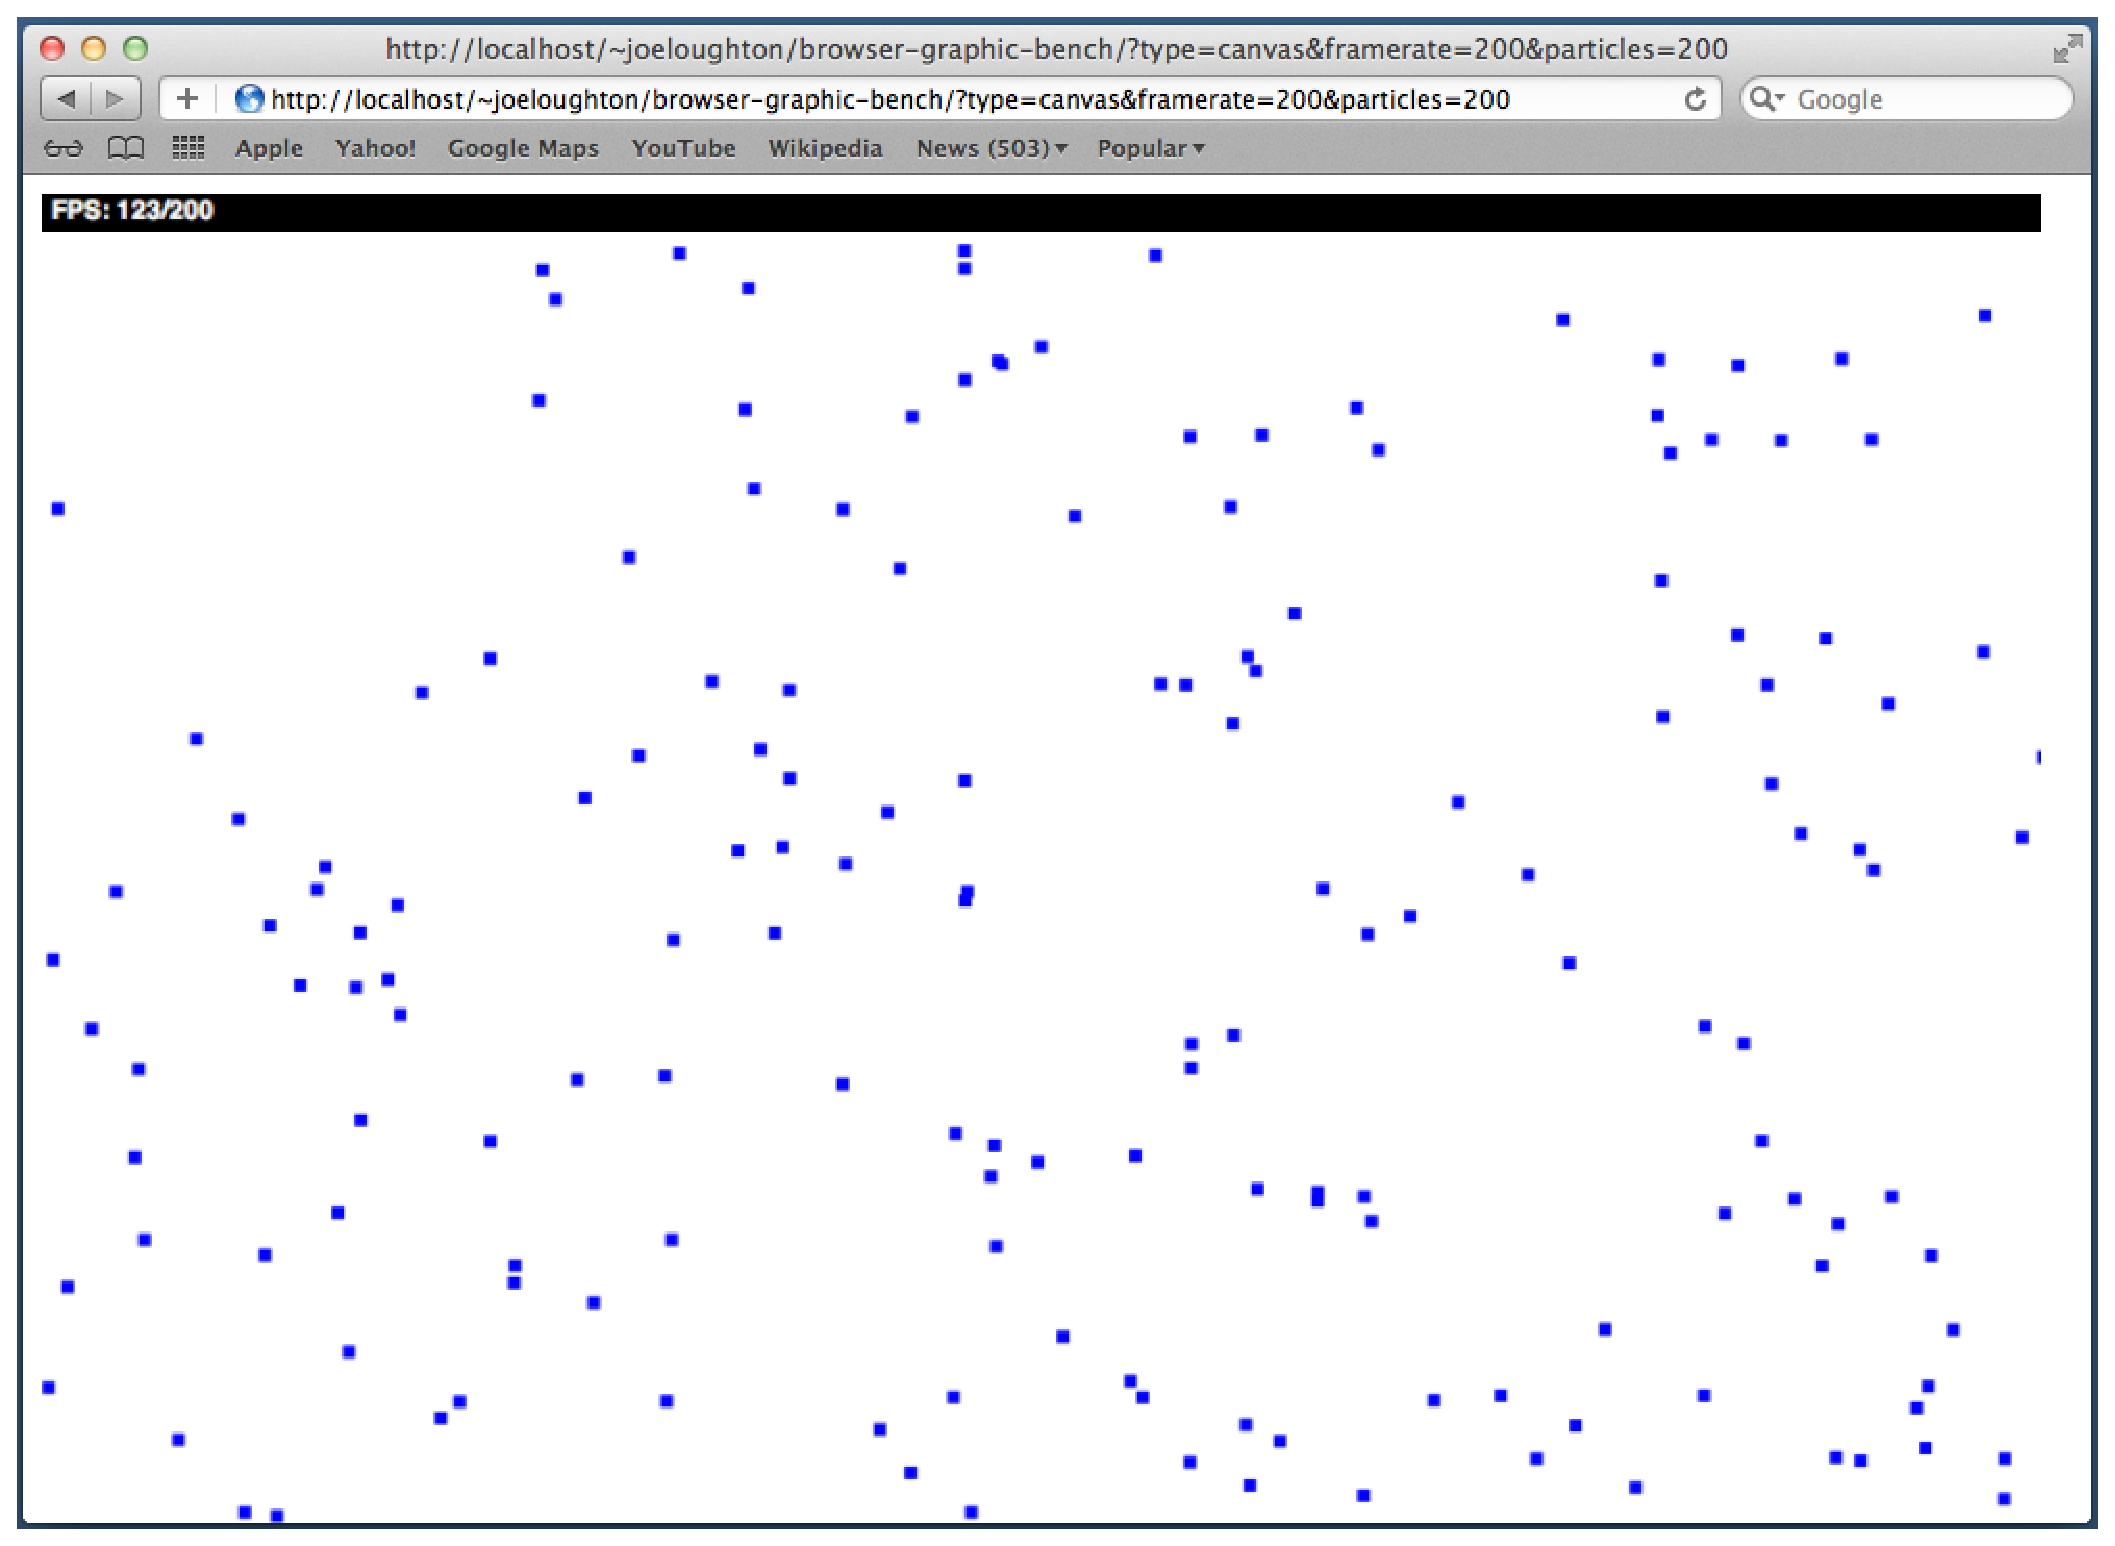
\includegraphics[width=170mm,height=130.08mm]{assets/benchmark-tool.eps}
\caption{The browser graphics benchmarking tool currently rendering 200
particles using Canvas and running in Safari. The potential frame rate using
this setup is shown to be 123.}
\label{fig:benchmark-tool}
\end{figure}

\begin{figure}
\centering
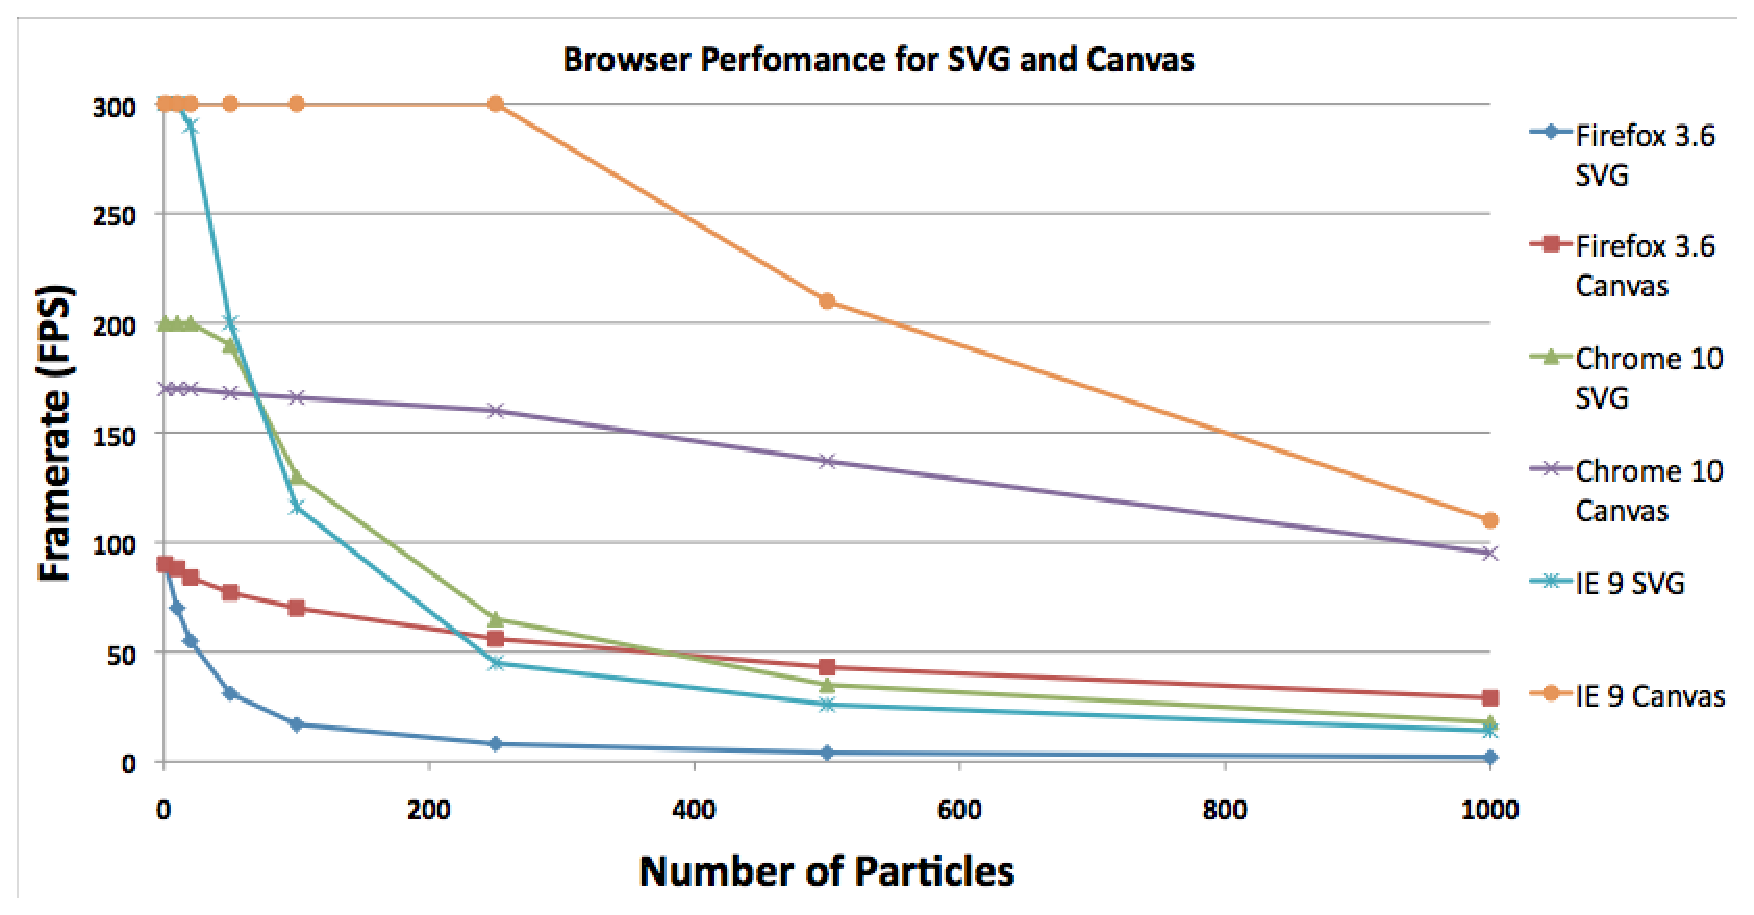
\includegraphics[width=170mm,height=91.67mm]{assets/benchmark-graph.eps}
\caption{The results of the graphic benchmark run on a Windows 7 host. Three
different browsers are tested using both SVG and Canvas.}
\label{fig:benchmark-graph}
\end{figure}

% Scalability issues
The two most widely supported and popular browser native technologies are
Scalable Vector Graphics (SVG) \cite{Ferraiolo_2003} and Canvas
\cite{Canvas_website}. SVG uses vector based graphics whereas Canvas is a bitmap
system. SVG allows vector objects to be created and added to the HTML Document
Object Model (DOM). User interaction such as mouse clicks can be easily added to
one of these objects and vector sets can be changed. Canvas on the other hand
requires the programmer to develop their own user interaction system and the
entire canvas must be redrawn when any change is required. It would therefore
appear that SVG was the most natural choice to go with for network maps that
require user interaction for nodes and edges. However, previous tests have shown
scalability performance problems with SVG \cite{Johnson_2008}. These tests are
four years old relative to this project so it was deemed necessary to develop a
benchmark tool to produce updated results.

The benchmark tool was developed using JavaScript to run across all modern
browsers. It generates a given number of rectangles and begins moving them
around the screen in random directions. The frame rate achieved for the current
number of rectangles and the given technology is displayed at the top of the
screen. See Figure \ref{fig:benchmark-tool} for an example of a running
benchmark. This tool was run on Windows and Mac computers across the latest
versions of the Firefox, Safari, Internet Explorer and Chrome browsers. 

% Maybe elaborate more here...
The results of the tests are shown in Figure \ref{fig:benchmark-graph}. At the
500 particle mark the top three lines are all Canvas based frame rates. SVG
performance is shown to drop significantly in the first 50 to 100 particles
where as Canvas achieves a much more level gradient. NetMapJs needs to be able
to visualise networks that will potentially have many more nodes than the
performance limits of SVG allow for. As a result, Canvas was chosen as the web
graphics technology for this visualisation. However, the graphics generation
system was kept separate from the rest of the code. This means that if
performance of these technologies shift in the future, a new graphic system
could be implemented and slotted in to reflect the change.


\subsection{Libraries}
\label{sec:libraries}
  % Go over the key libraries used
  %   > eg jQuery, Javascript Infovis Toolkit, arbor, QUnit
  % Why did I choose these libraries
  % How did I pick them?

NetMapJs makes use of the jQuery, JavaScript InfoVis Toolkit and Arbor libraries
in its design. JQuery was used for several reasons \cite{jQuery_website}. Cross
browser support is important to ensure that each user gets the same experience
across different systems. JQuery functions are portable and are especially
useful for eliminating browser specific code. JQuery also simplifies HTML
document manipulation, event handling and AJAX interactions. The JavaScript
InfoVis Toolkit provides a framework for producing interactive, web based
visualisations \cite{thejit_website}. The toolkit includes many useful features
such as node-edge graph manipulation functions, complex number arithmetic,
animation transitions and so on, which are needed for this project.

NetMapJs includes some automatic layout algorithms for initially deciding where
to position nodes in the network map. One of these layouts is a force directed
algorithm. This are a class of algorithms that lay out the graph in an
aesthetically pleasing way by applying forces to nodes and edges. The Arbor
JavaScript library was used for this as it performs well and provides mechanisms
for changing physics parameters such as gravity and friction
\cite{Arbor_website}. The QUnit library is a unit testing library plug-in for
jQuery. This assisted with test driven development during the implementation
stage of the project.

\newpage

\section{Visual Design} 
\label{sec:visual-design}
  % Overview of visual design

In this section, the most significant design aspects of NetMapJs are explained.
Justification for each of the design decisions is given along with example
screen shots taken from NetMapJs views.

\subsection{Nodes}
\label{sec:nodes.vis}
  % Design considerations for nodes
  % Nodes can be sub networks
  %   > Helps for scalability
  % Grouping, hiding nodes
  % Combining with symantic zooming
  % Screenshots

  % What are nodes with respect to network maps?
  % What are subnetworks?
  % How have I combined the two?
  % Screenshot 1
  % What is the advantages of this?

Nodes in network maps are traditionally used to express a particular physical or
virtual device. Nodes are joined together by edges which represent the
relationship or connection between then. Subnetworks are a specific group of
devices that relate to each other by a common subnet. Subnetworks may consist of
other subnetworks of their own and altogether they can be seen as a single
network. It is possible to apply this concept to nodes when designing a
visualisation. Nodes can visually contain sub nodes and so on for a given number
of depth levels. Nodes that fall into this category will be referred to as
group nodes.

Figure \ref{fig:nodes1.0} shows the Hamilton (HLZ) PoP for the KAREN network.
The outer circle marks the HLZ node and the smaller, solid circles inside
illustrate the sub nodes of that PoP. This grouped effect causes the viewer the
assume that the sub nodes are related to each other through a common parent
node. Figure \ref{fig:nodes1.1} shows a zoomed in view of the same HLZ group
node. The parent node and edges are now faded out so that the focus is now on
the sub nodes and edges. This idea of zooming and adding detail is explained in
Section \ref{sec:navigation.vis}. The layout of the sub nodes within a group is
also an important design decision as different group nodes may make sense to be
laid out differently. The HLZ group node is using a star layout. Layout
considerations are discussed in Section \ref{sec:layouts.vis}.

  % May want to see nodes only at a given level...
  % How have I done this?
 
\begin{figure}
\centering
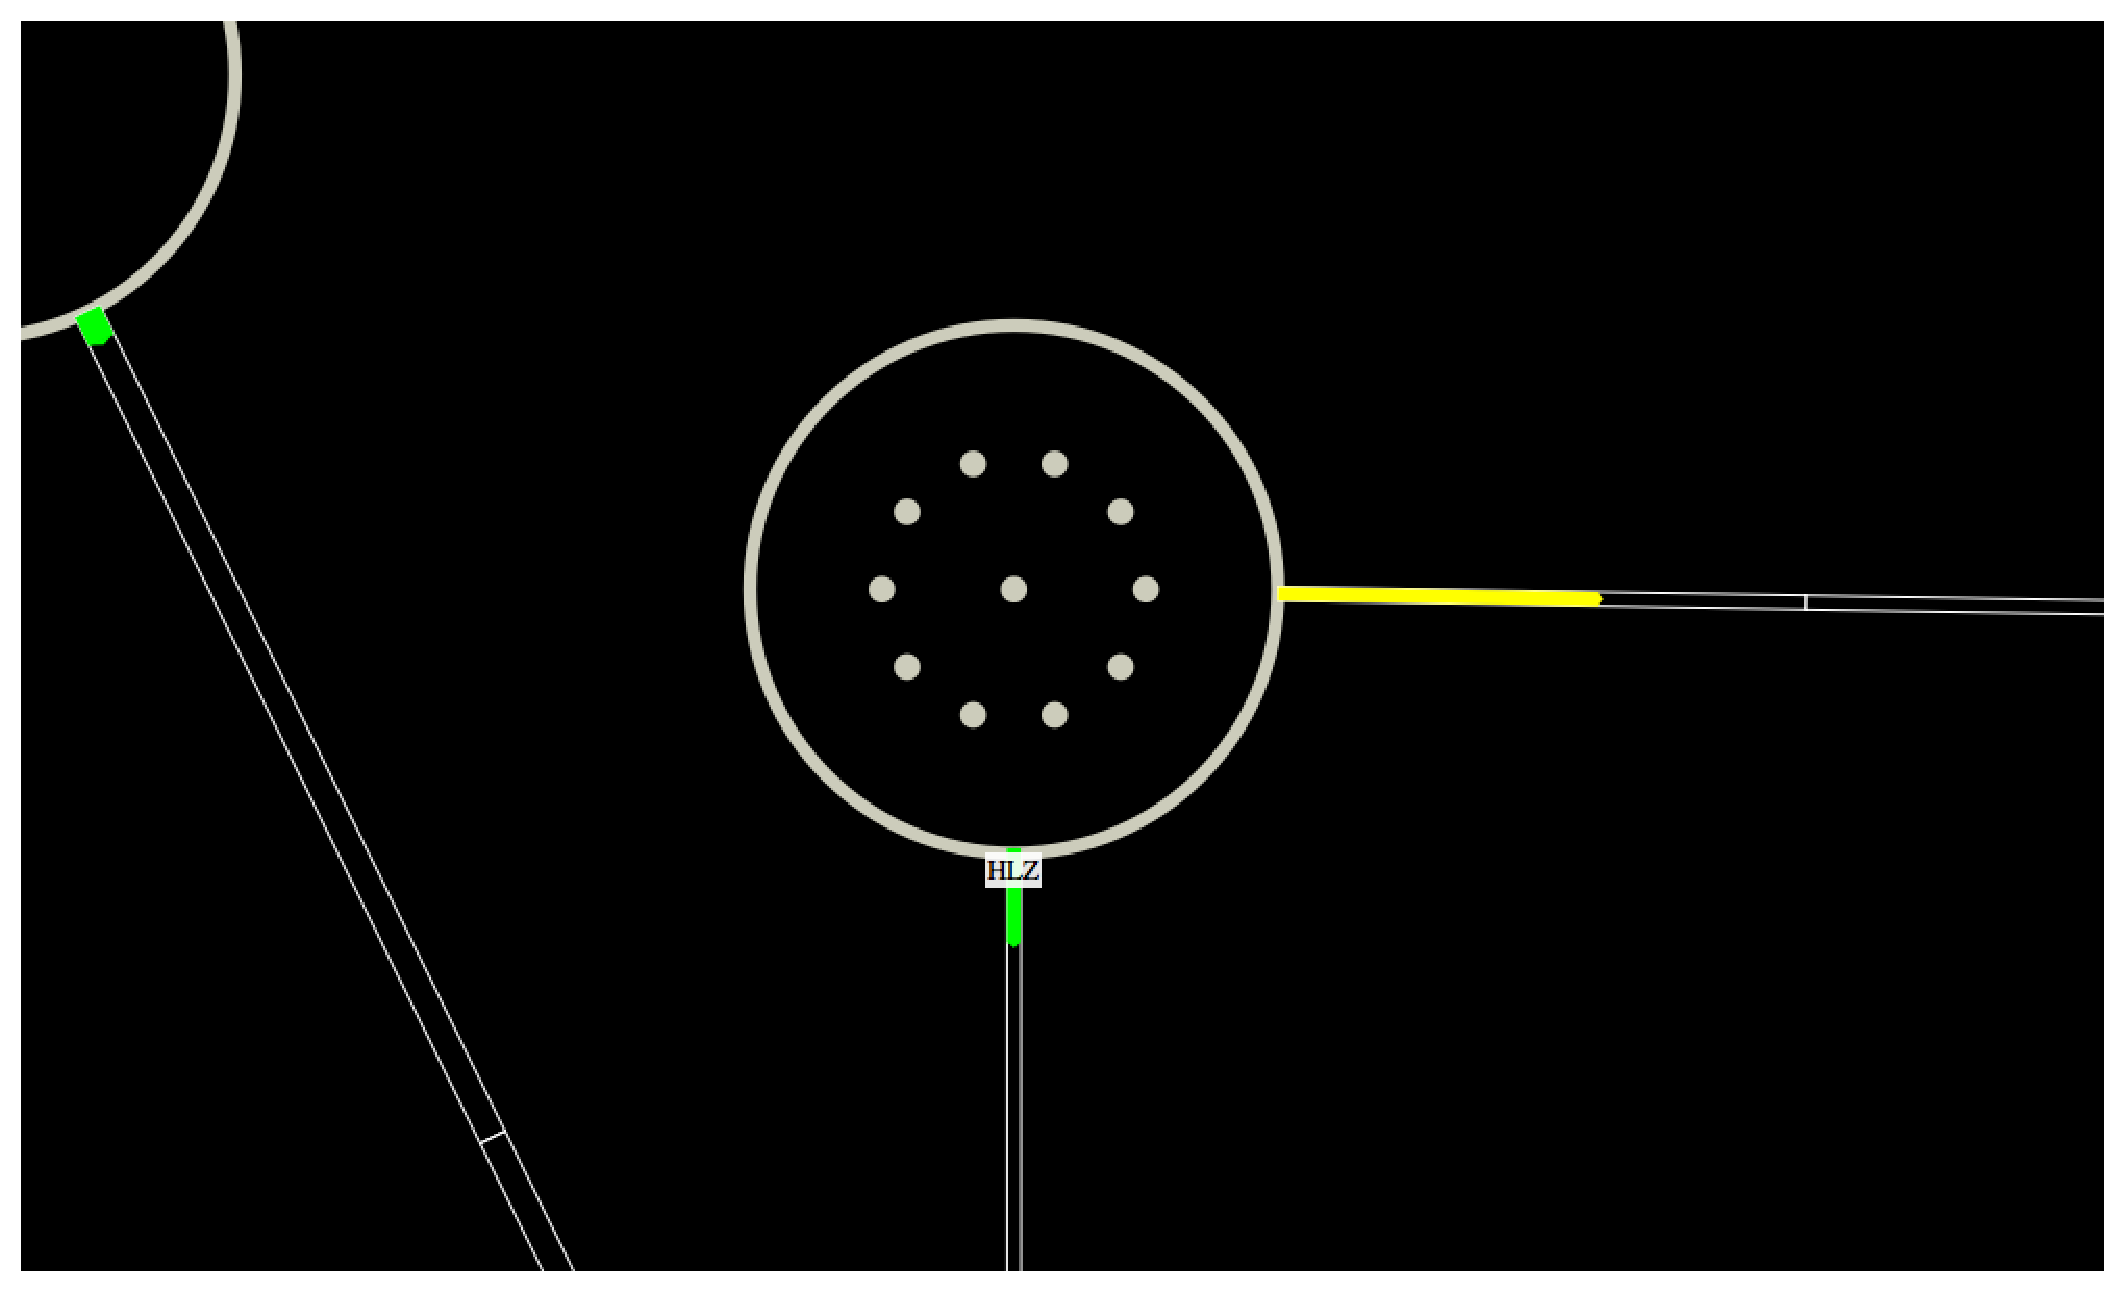
\includegraphics[width=170mm,height=107.58mm]{assets/nodes1-0.eps}
\caption{A section of the KAREN network map that shows the Hamilton (HLZ) PoP
node.}
\label{fig:nodes1.0}
\end{figure}

\begin{figure}
\centering
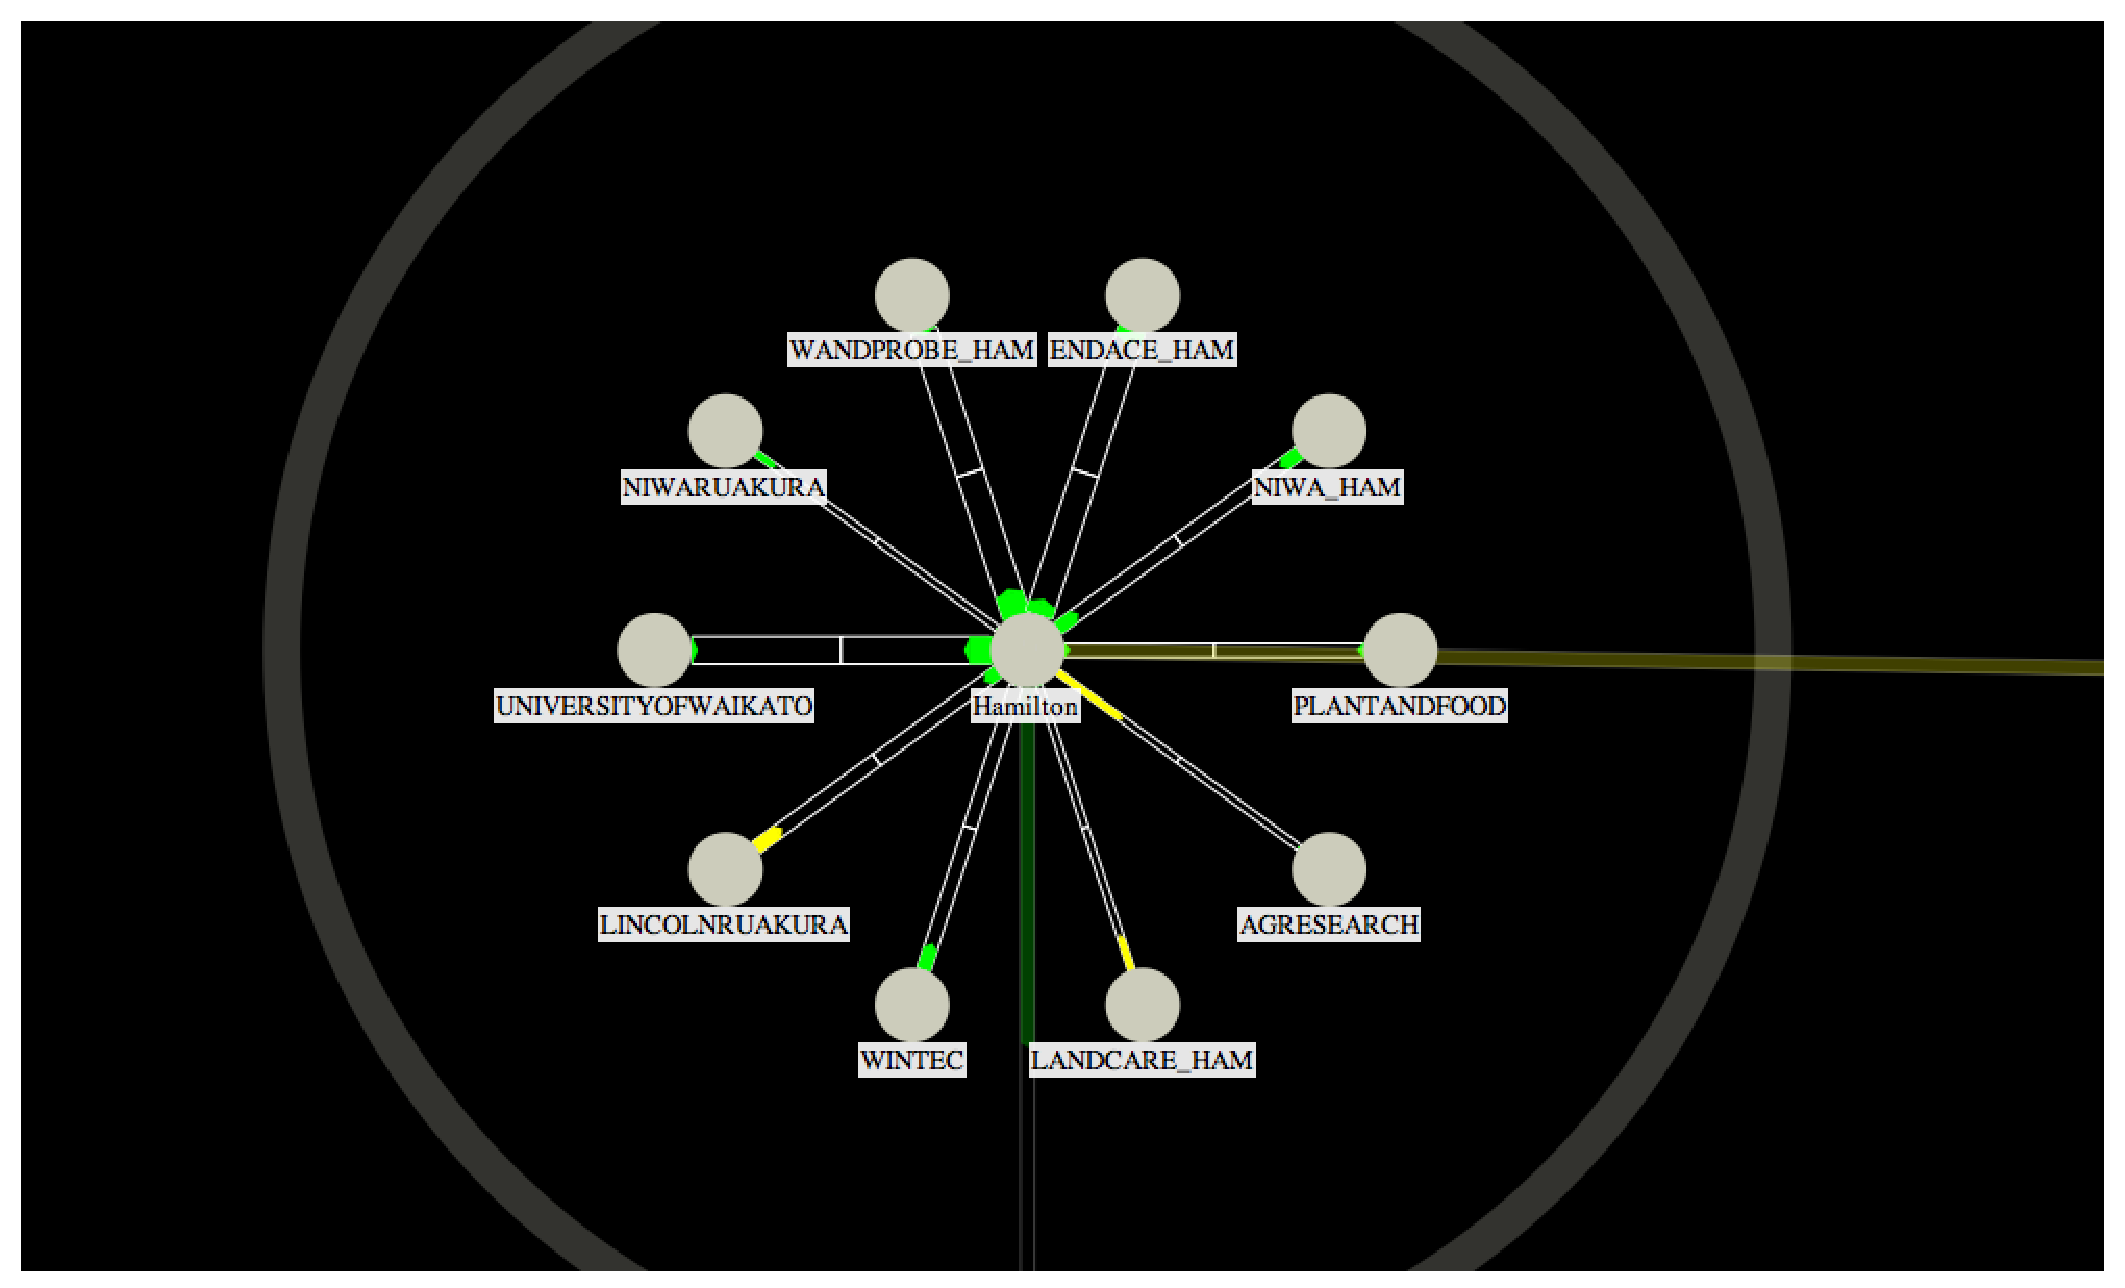
\includegraphics[width=170mm,height=101.93mm]{assets/nodes1-1.eps}
\caption{A zoomed in view of the HLZ PoP that shows its children nodes.}
\label{fig:nodes1.1}
\end{figure}

\subsection{Edges}
\label{sec:edges.vis}
  % Simple line between two nodes
  % Can make use of this space more effectively
  % Explain the visual design of my way
  %   > visualisation principles included
  %   > Quantitative vs qualitative
  % Screenshots

Edges between nodes in a network map indicate that two or more devices are
connected to each other by some medium. A single line between two nodes is
enough to show this relationship. If this line is thin then it reduces the
amount of clutter for the same number of edges \cite{Tufte_2007}. Figure
\ref{fig:edges1.0} shows the display of a network with many nodes using thin
lines.
% TODO: fill out paragraph more?

In the case of network maps, there is often monitoring data available that
directly relates to the performance of a given edge medium. This data could be
accessed through a separate view in the visualisation but there are advantages
to showing this directly on map. For example, if something goes wrong with a
link then an indication on the main view on the visualisation will attract the
user's attention immediately as opposed to the case where the user had to follow
some interaction sequence to access the data. For this project, a new way of
visualising quantitative variables describing a bidirectional network connection
was developed. In particular, this method suits variables which have an upper
limit such as the bandwidth or packet loss of a link.

Figure \ref{fig:edges1.1} gives an overview of how the connection visualisation
works by using bandwidth as an example. A rectangle is drawn between two nodes
and split at the mid point. The side of the split rectangle closest to a given
node represents the direction from that node to the destination. The height of
each of the rectangular sections indicates the total quantity of the variable.
For bandwidth, this would be the total for that direction of the link and may be
different to the other direction in the case of asymmetric connections. Arrows
extend from a given node towards another with the length being relative to the
percentage of the variable's proximity to its upper limit.  The colour of the
arrow is based on some user defined categorical variable such as the health of
the network link.

The design for this graphic took careful consideration of information
visualisation principles. Position and length are the most accurate methods for
encoding quantitative variables \cite{Spence_2007}. The design uses length to
show total and percentage utilisation. The use of position is also shown in the
arrow as a proportion of the total rectangular section. Colour hue is effective
at displaying categorical variables which is how it is being used in the
visualisation. Figure \ref{fig:edges1.2} shows this design implemented in
NetMapJs and is being used to show the bandwidth between the Palmerston North
and Wellington PoPs in the KAREN map.

\begin{figure}
\centering
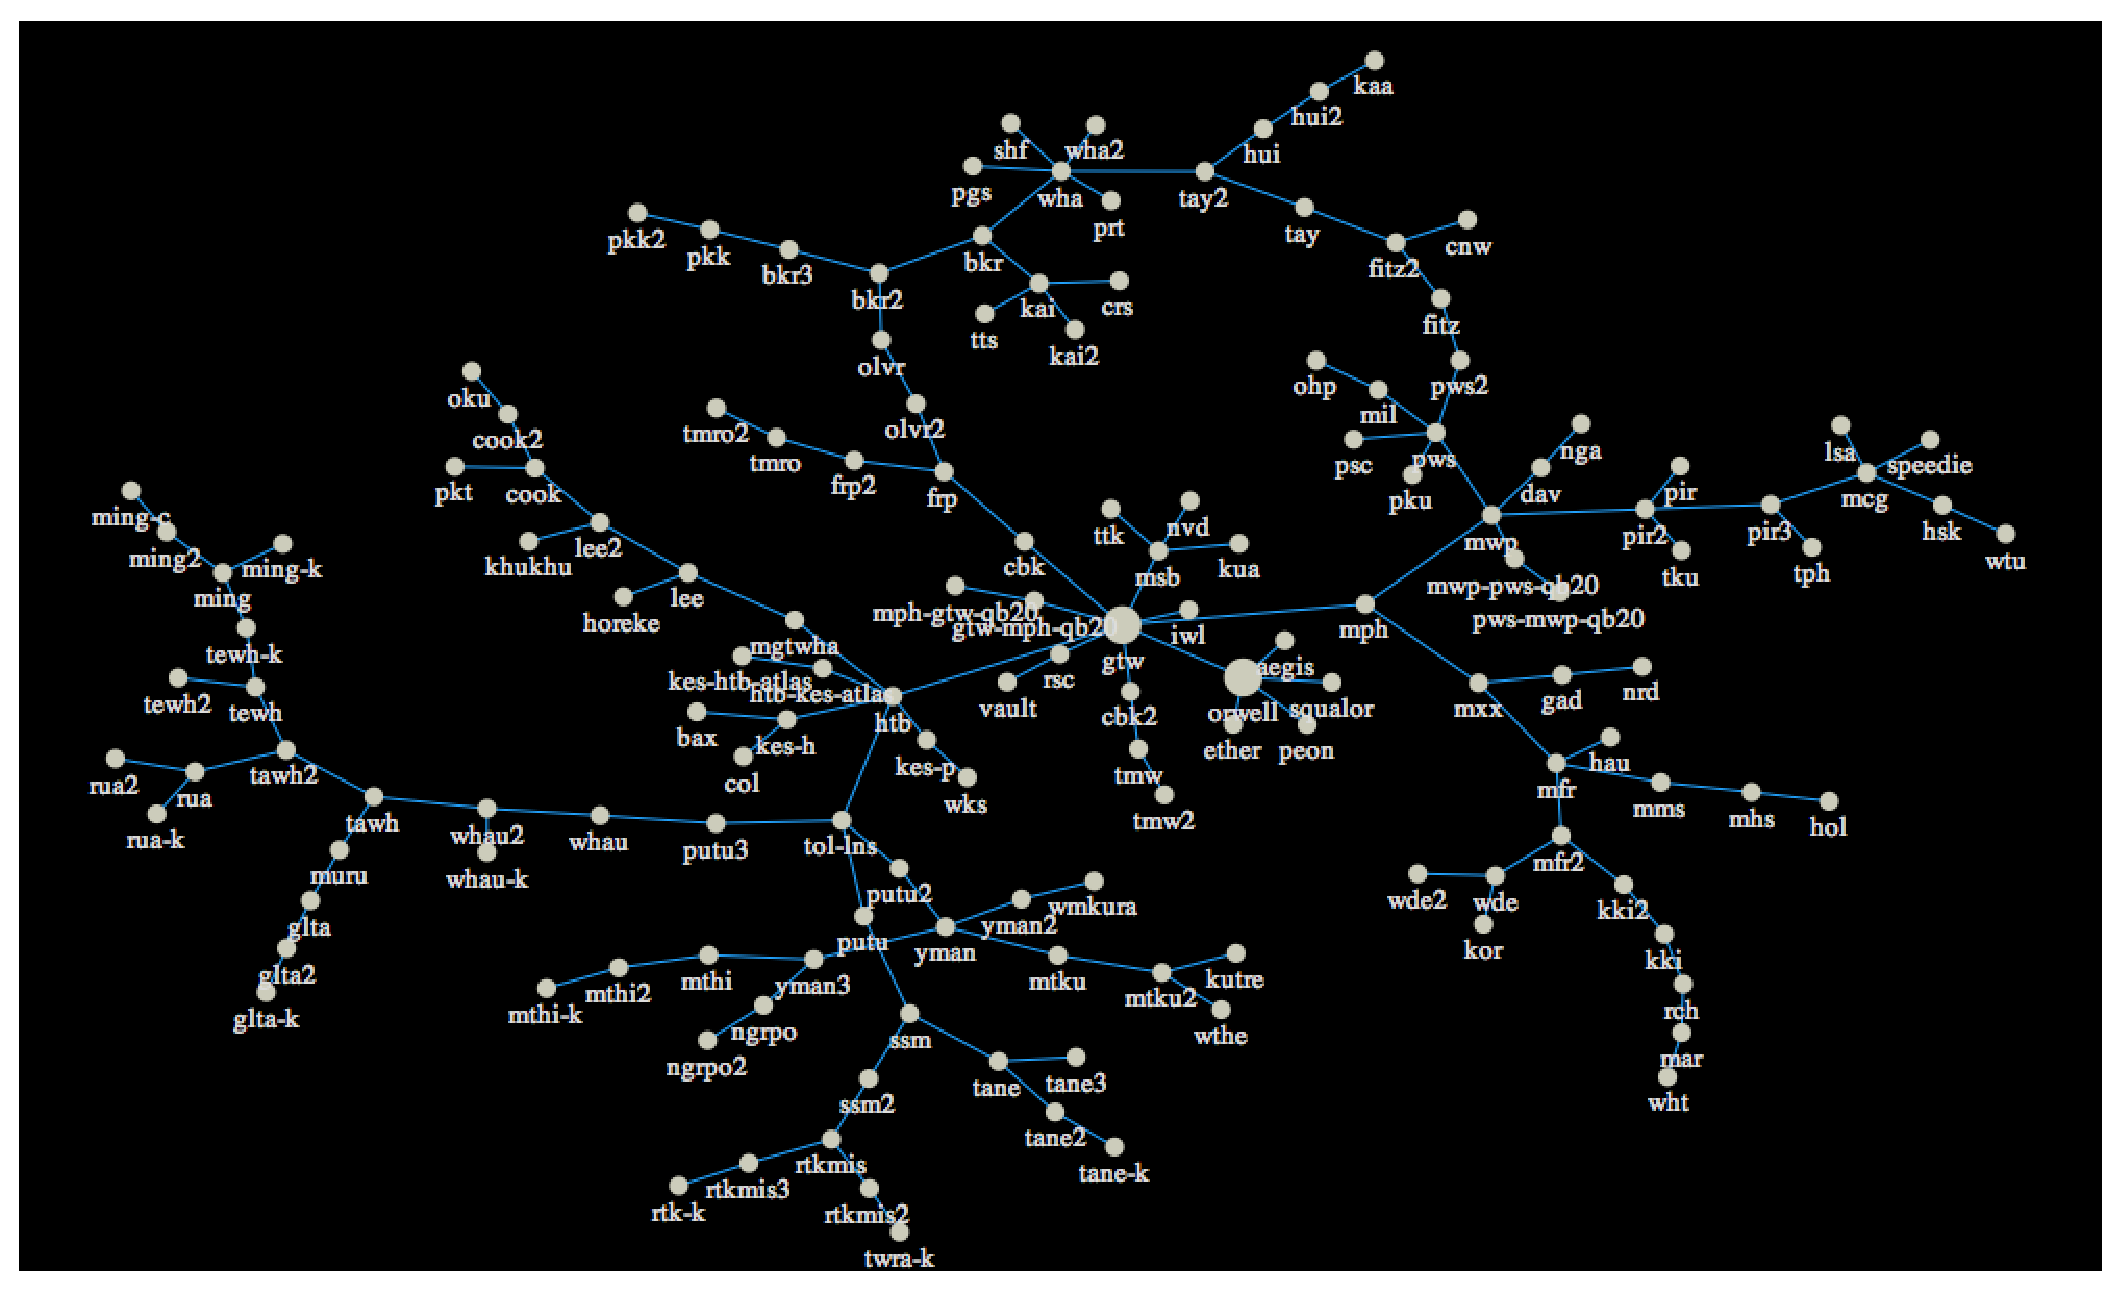
\includegraphics[width=170mm,height=102.54mm]{assets/edges1-0.eps}
\caption{An overall view of the Rural Link network. Nodes are positioned to
reduce edge crossings using a force directed layout.}
\label{fig:edges1.0}
\end{figure}

\begin{figure}
\centering
\includegraphics[width=170mm,height=59.03mm]{assets/edges1-1.eps}
\caption{A diagram showing how edge data can be visualised effectively.}
\label{fig:edges1.1}
\end{figure}

\begin{figure}
\centering
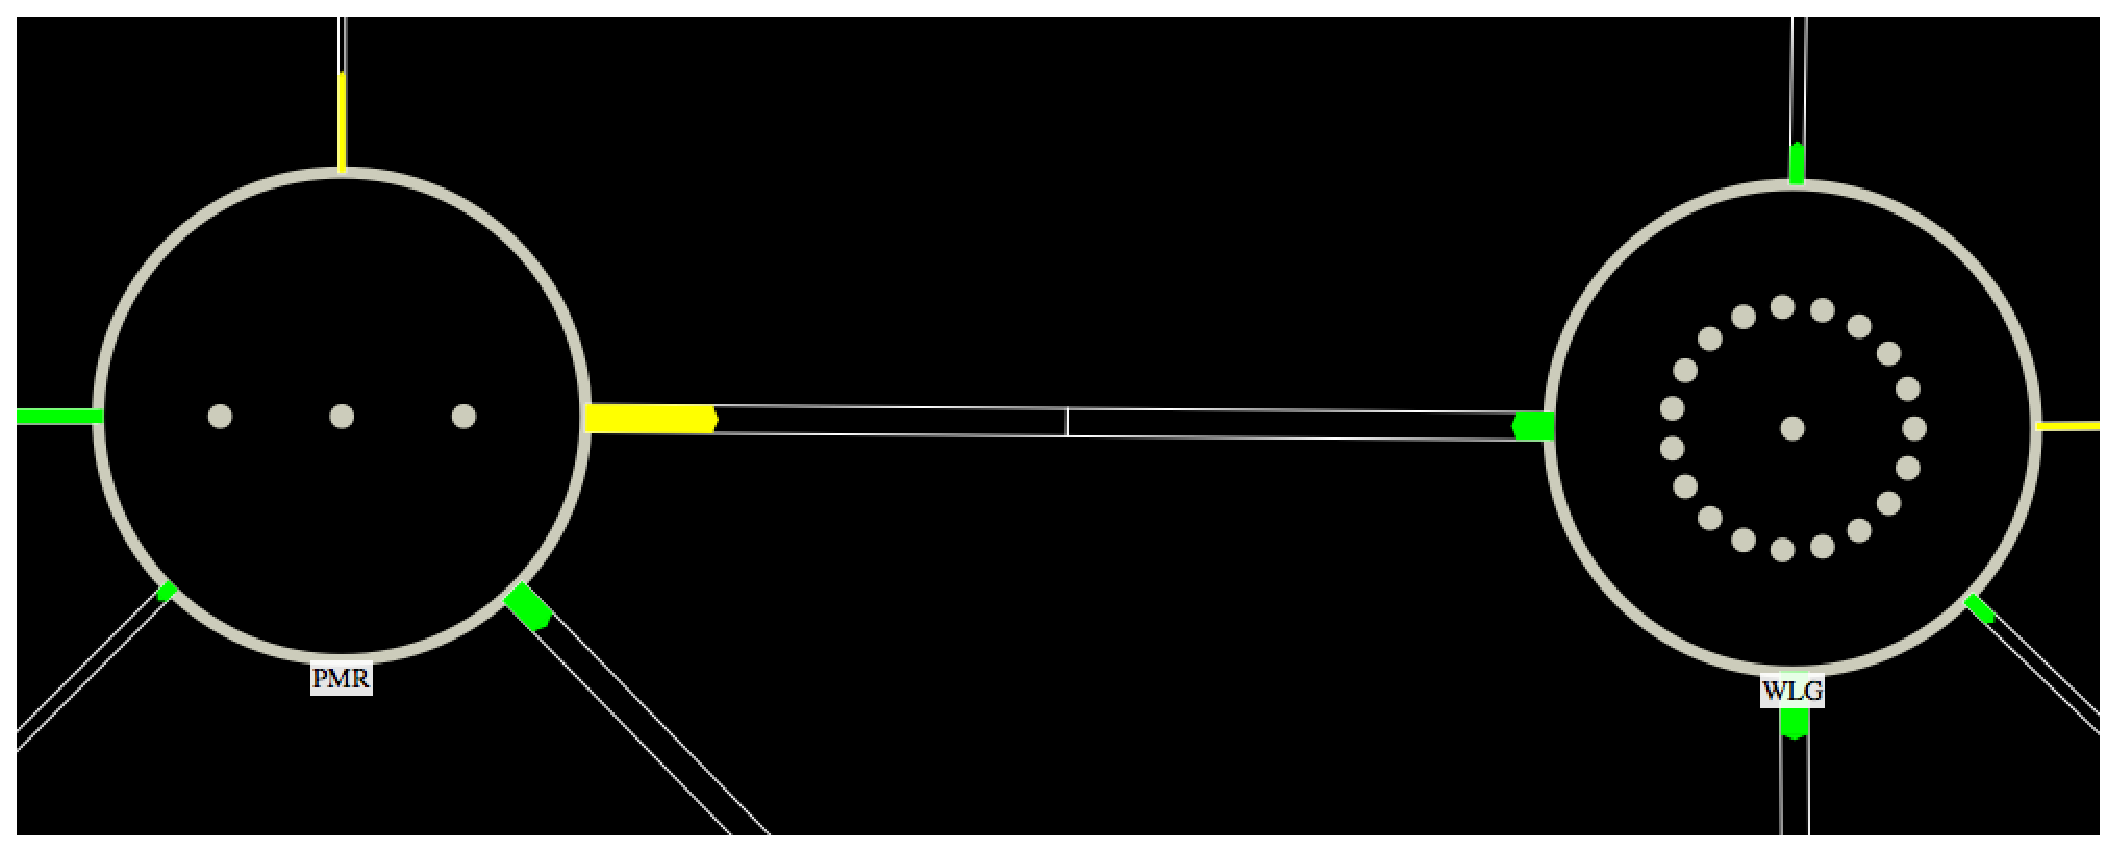
\includegraphics[width=170mm,height=70.21mm]{assets/edges1-2.eps}
\caption{The new edge design shown within NetMapJs. The edge is connecting the
Wellington and Palmerston North PoPs in the KAREN network.}
\label{fig:edges1.2}
\end{figure}

\subsection{Layouts}
\label{sec:layouts.vis}
  % Explain importance of node layout
  %   > Different subgroups - different layouts
  %       - reference Java3D paper - has lots of layout talk
  %   > Groups have layouts
  % Which layouts did I implement and why
  % Screenshots

% importance
%   > Too much time required to statically layout large networks
%   > Need to minimise overlapping
%   > Need to maximise user understanding and recognition
%   > Good layout can lead to greater understanding where as bad can be
%   missleading
% “Finding the Best Viewpoints for Three–Dimensional Graph Drawings
% 

% Herman_1998 - great graph layout issues as well as focus, context techniques
% and zoom//pan issues.
% Graph Visualization and Navigation in Information Visualization
% 

A good layout of nodes in a network map is important to maximise the insight and
understanding possible to the user. A bad layout can lead to the cluttering of
nodes and edges or, worse, a misunderstanding of the underlying data. The use of
3D layouts provide more available space for positioning nodes but can introduce
new problems. Nodes and edges in a 3D layout may occlude other objects and it is
hard to choose an ideal perspective within the 3D space \cite{Lai_1998}. 2D
layouts are used in this project which simplifies the use of semantic zooming as
described in Section \ref{sec:navigation.vis}. 

Two basic 2D layout algorithms were used in this project in addition to
statically defining node positions. A force directed and star algorithm. These
two were chosen because they were known to work well with the example datasets
and provide a good starting point over just static layouts. A complete network
map tool would include many more layout algorithms to cope with a wider range of
network layout structures \cite{Paul_2000}. Figure \ref{fig:edges1.0} shows
Rural Link's network laid out using the force directed algorithm. The algorithm
lays out the network particularly well due to its tree like structure. In
particular, there are no overlapping edges or nodes in the map. Redundant
connections are shown clearly by branches that join up to form a loop. 

Sub groups may make sense to have separate layout algorithm applied to them when
the underlying network structures are different. An example of this is
demonstrated in Figure \ref{fig:layouts1.1}. The overall view of the KAREN map
contains statically defined node positions that are based on layout designs by a
graphic designer. When the user zooms in to a particular PoP, it can be seen
that the layout of that group is a star layout. One central node, the
distribution router, connects to all the other devices in that PoP, making the
star layout particularly appropriate for displaying subnetworks at the PoP
level.

\begin{figure}
\centering
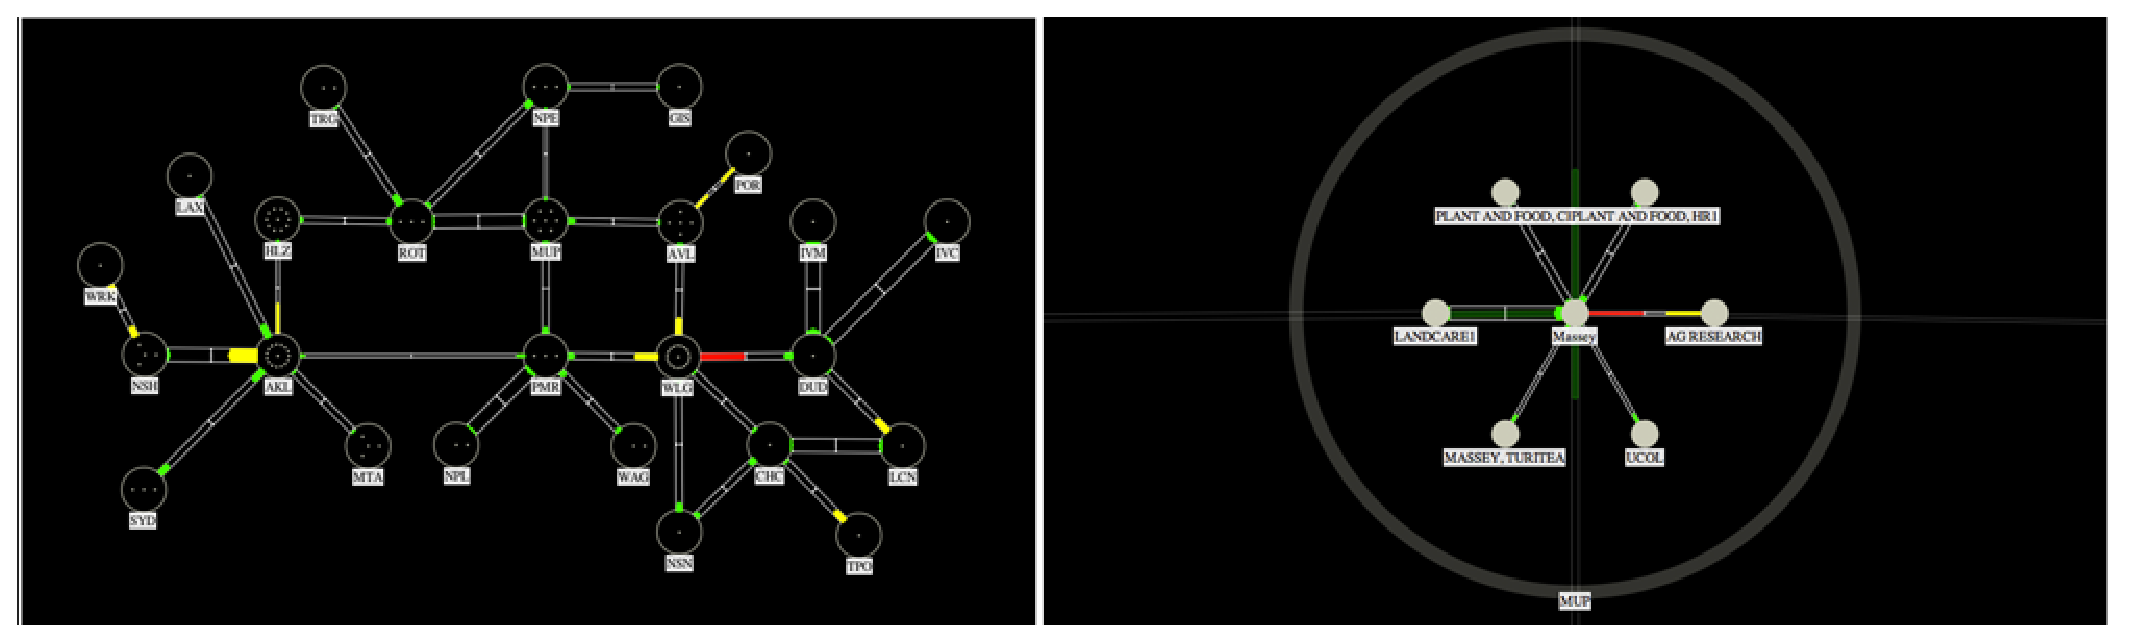
\includegraphics[width=170mm,height=49.34mm]{assets/layouts1-1.eps}
\caption{An overall view of the KAREN network is on the left that uses a static
layout. On the right is a zoomed in view that shows the Massey sub group having 
a star layout applied.}
\label{fig:layouts1.1}
\end{figure}


\subsection{Navigation}
\label{sec:navigation.vis}
  % Details of navigation
  % Why is getting it right important
  % Issues relating to navigation
  % Zoom, pan, zoom/center nodes, follow edges
  % Screenshots

Layout algorithms can be good displaying large graphs clearly but there is a
limit to their effectiveness. At some level of network size or density the
limits of these algorithms will be reached and ideal layouts will no longer be
guaranteed. It is also likely that a user can not even decipher information and
patterns from such large networks. It is therefore useful to combine layout
algorithms with other techniques in order to remain scalable \cite{Herman_2000}.
Grouping devices into subnetworks is a reduction technique that is further
described in Section \ref{sec:nodes.vis}. 

Another technique for reducing networks is semantic zooming \cite{Perlin_1993}.
This is different from geometric zooming in that changes are made to the level
of information displayed while moving towards a specific area of a graph. What
would perhaps be visually overwhelming if presented all at once, can instead be
drip fed to the user as they indicate that they are more interested in a
particular subsection of a network. NetMapJs uses semantic zooming along
with panning to effectively navigate throughout large networks. 

Figure \ref{fig:nav1.0} shows more detail being revealed to the user as they
zoom in to a sub group of the KAREN network. In the fully zoomed out view it is
important to indicate that there is distant content so that the user is aware
that they can zoom in for further detail \cite{Spence_2007}. Sub groups indicate
that they contain more detail by using small dots and as the user zooms in to
that group, more detail such as labels and edges between nodes appear. At this
point, the group node graphic and its external edges become faded out which
allows the user to focus more on the current group's detail while still being
aware of the group that the nodes belong to.

While implementing the design of NetMapJs, it became apparent that it was
increasingly difficult to navigate between nodes in the map as you zoomed deeper
into sub groups. For example, when zoomed into the Hamilton PoP in the KAREN
map, it would require a lot of user interaction to view the directly connected
Auckland PoP. Several drags of the mouse would be required to pan towards
Auckland. To eliminate this problem, two navigation features were added.

The first feature enables the user to follow an edge to the node on the other
end in one click. For example, if the user is currently zoomed in to the
Hamilton PoP and wants to go to the Auckland PoP, they can simply click the edge
that connects the two. An event triggered tooltip is displayed over an edge to
notify the user of the node that lies on the other end of it. This is shown in
Figure \ref{fig:nav1.1}. The addition of animated transitions between view
changes allow users to keep context and to absorb the change
\cite{Lamping_1995}.  NetMapJs uses animation this way to transport the user to
the new view such that they get a sense of where in the network they are moving
to. A direct jump from the source to destination node risks confusing their
perceived location in the overall network.

The other feature for improving navigation is zooming and centering nodes.
Originally, when a user knows that they want to view a particular group node
normally, they would perform a sequence of zooming and panning actions to bring
it into focus. This feature allows the user to simply right click on a group
node to automatically bring it into focus again using animation to change the
views. Figure \ref{fig:nav1.2} demonstrates this effect. Combining the two
features means that zooming and panning are not strictly necessary and allow the
user to freely move around the network map quickly and effectively. The manual
controls are still useful to make minor adjustments to the view and to zoom back
out.

\begin{figure}
\centering
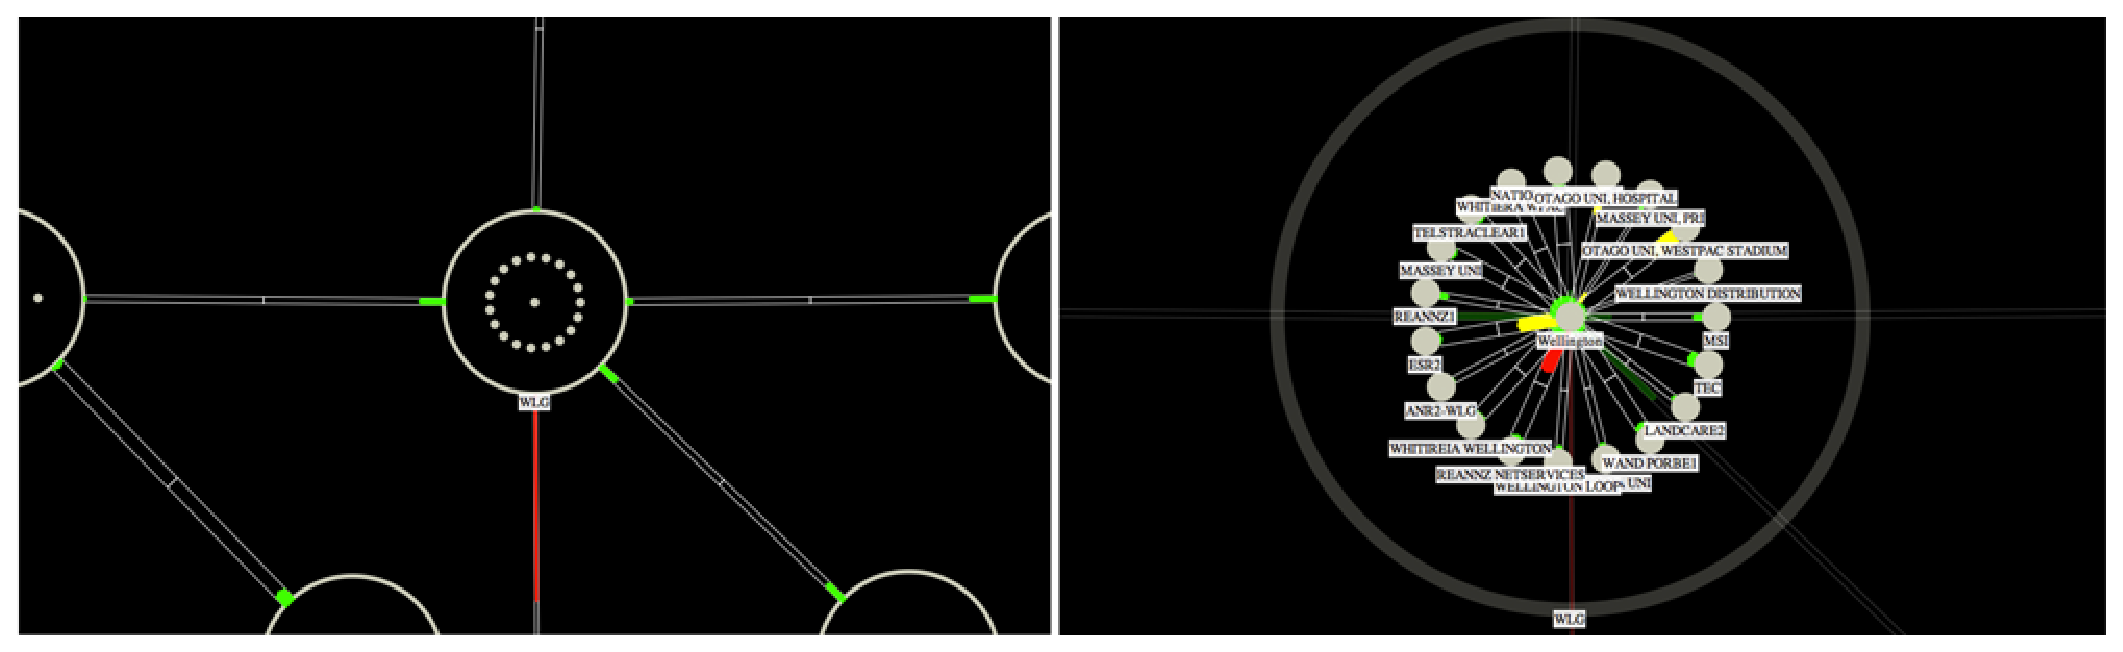
\includegraphics[width=170mm,height=53mm]{assets/nav1-0.eps}
\caption{The view on the left shows an indication of more detail within the
Wellington PoP. The zoomed in view shows the addition of more details such 
as edges and labels}
\label{fig:nav1.0}
\end{figure}

\begin{figure}
\centering
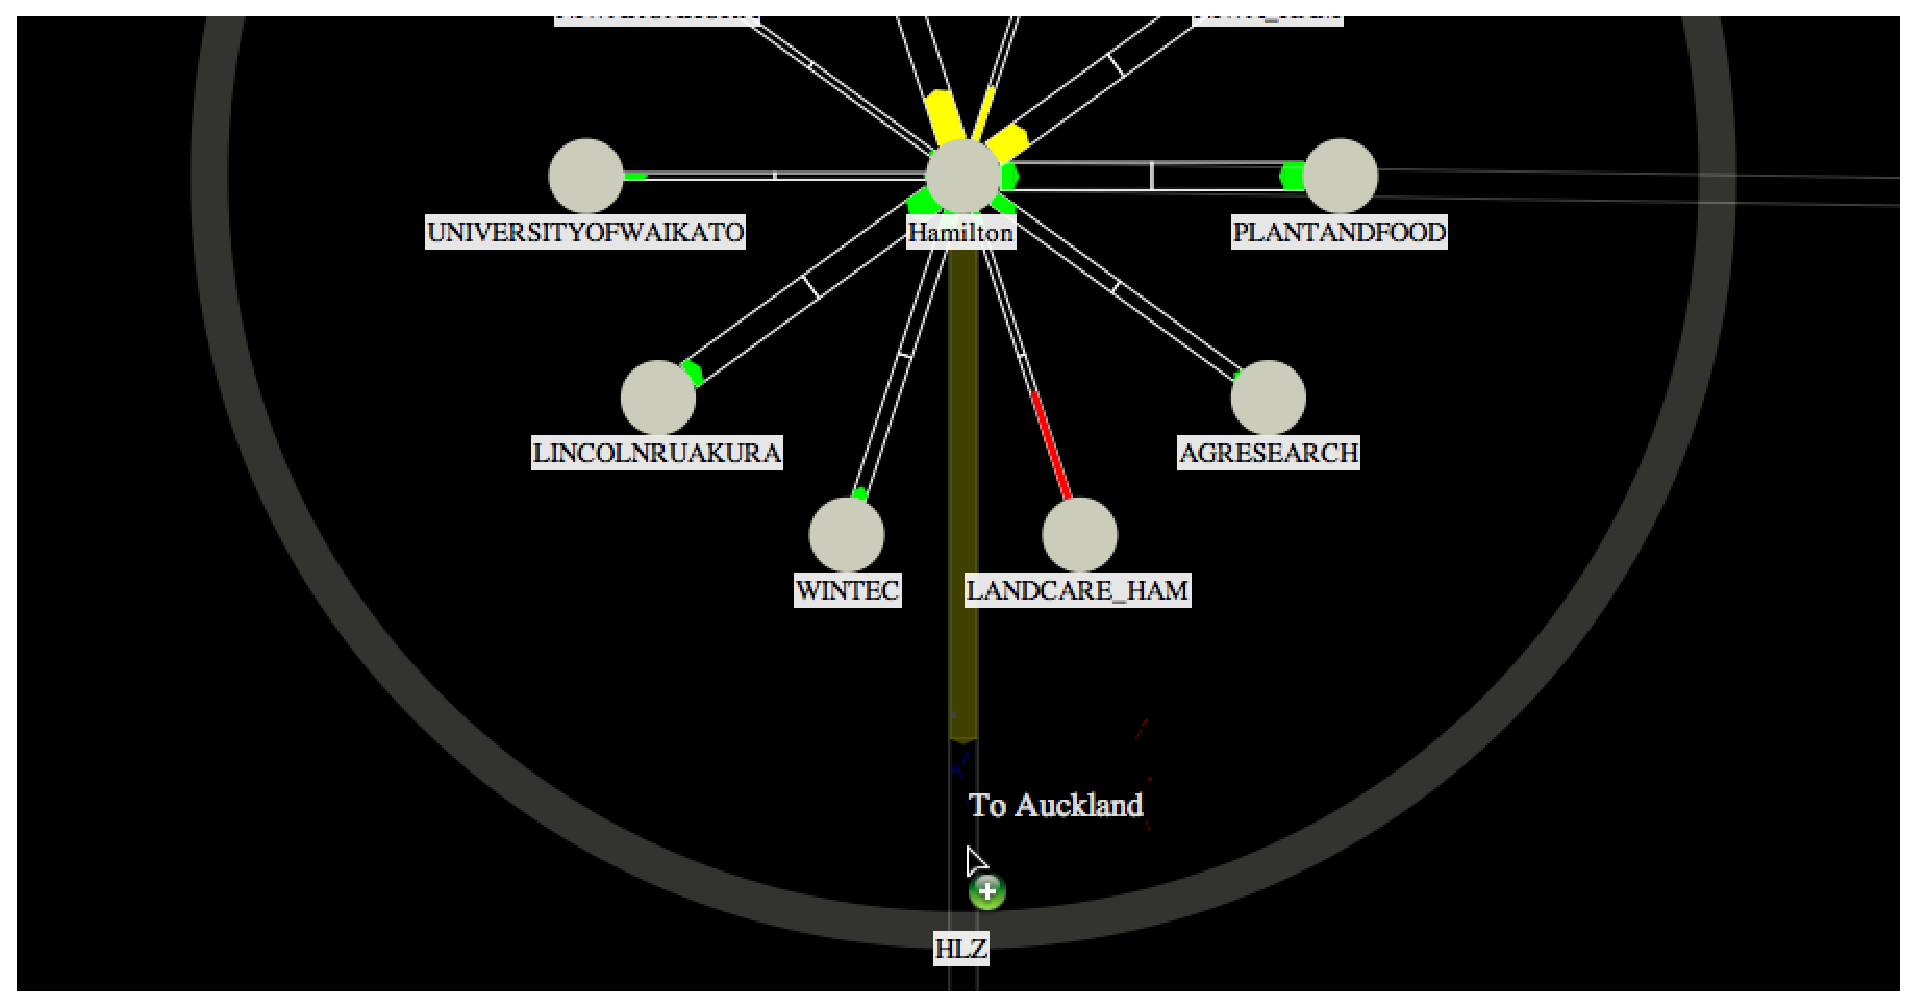
\includegraphics[width=170mm,height=88.01mm]{assets/nav1-1.eps}
\caption{A tooltip is shown by the mouse pointer that indicated where the user
will end up if they click on the edge.}
\label{fig:nav1.1}
\end{figure}

\begin{figure}
\centering
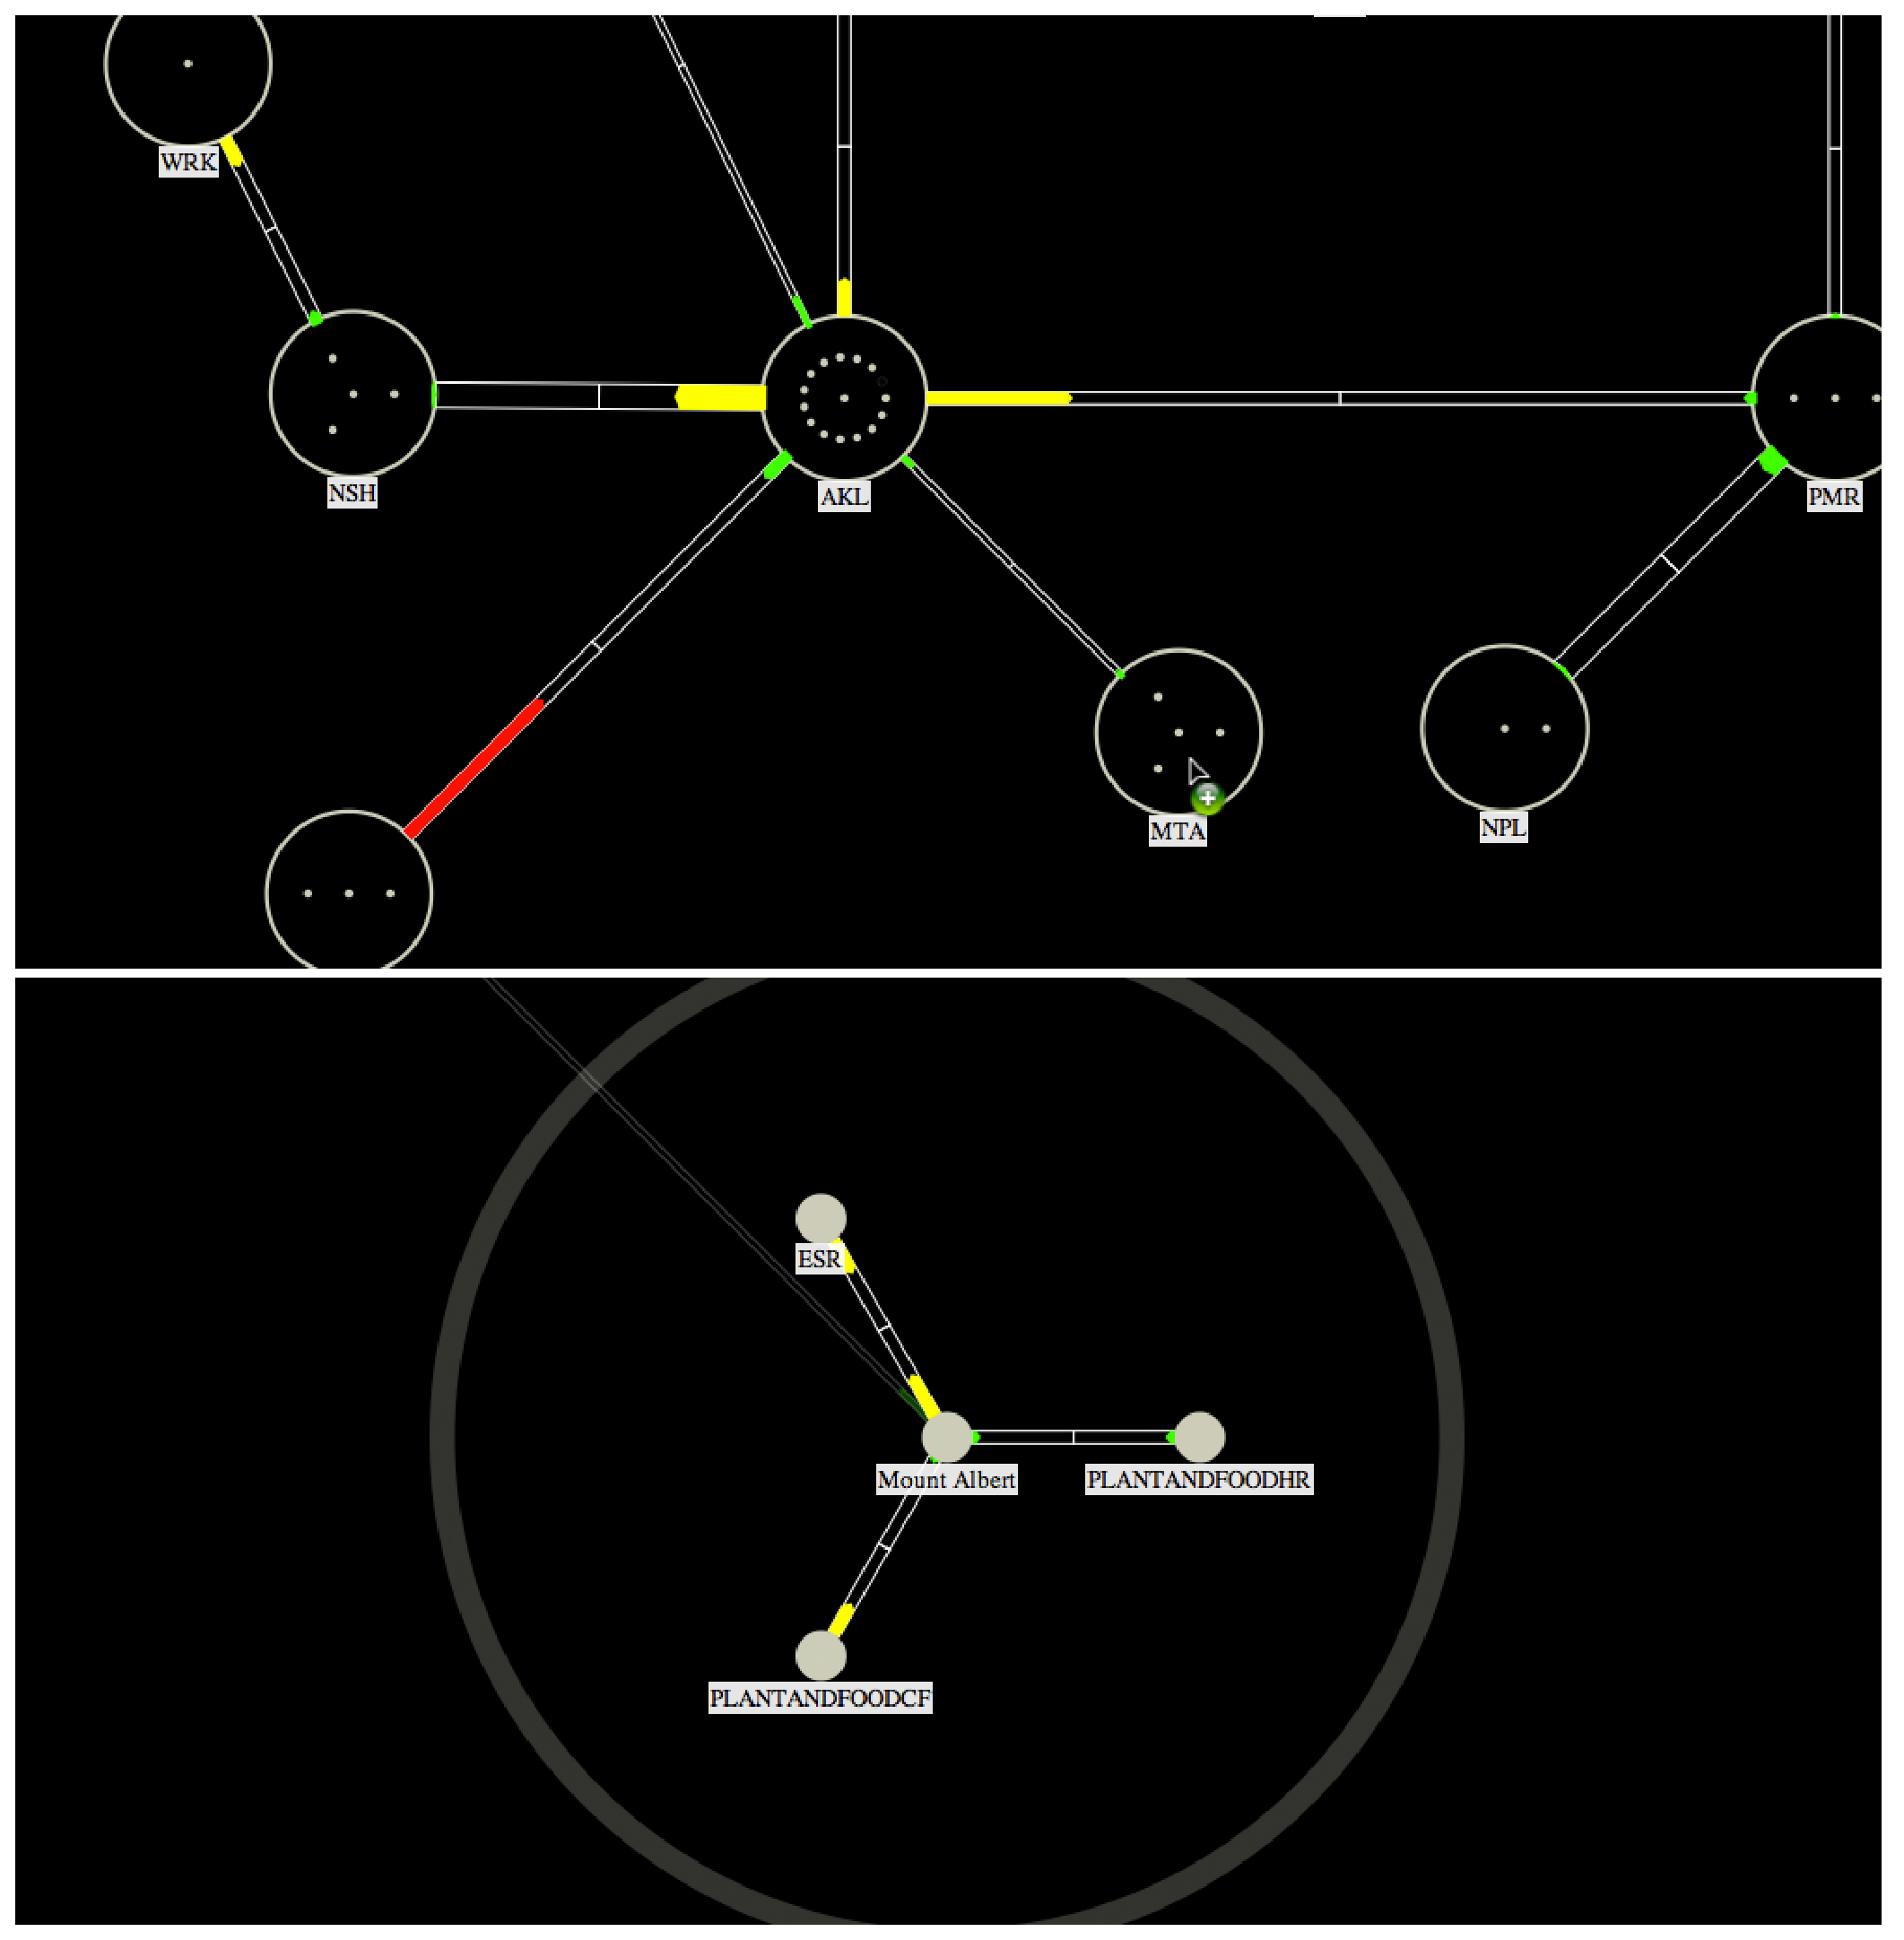
\includegraphics[width=170mm,height=173.22mm]{assets/nav1-2.eps}
\caption{The top view of the KAREN map shows where a user is clicking. The bottom
view shows where they would end up after the animated movement.}
\label{fig:nav1.2}
\end{figure}

\subsection{Overviews}
\label{sec:overviews.vis}
  % The problem - 
  % How is it solved - 
  % What does it look like - 
  %   > 

As a user zooms in to deeper levels of the network map, it becomes easy for them
lose context about where in the overall network they are. It is not ideal
for the user to have to zoom out just to regain this context. To address this,
NetMapJs makes use of multiple overview maps that each display a particular
level of the network. A level is defined as a zoom range in which no detail is
added or removed. Starting from an initial zoomed out view, as the user zooms
into a sub group of the network, a separate overview map for that level is added
to a stack of overviews. As the view port gets deeper into the map, more and
more overviews are added into this stack. When the user zooms back out, the
reverse happens and overviews are removed from the stack.

Figure \ref{fig:overviews1.0} demonstrates this stacking effect. Also visible in
the screen shot are yellow rectangles that have cross-hairs intersecting the
middle. The outline of the rectangles show where exactly the user's view port is
situated in the map as a whole as well as in each individual level. A cross-hair
was used to make sure the view port location can still be identified at higher
levels where the rectangle becomes too small to see. The overviews are also
linked to the main visualisation such that the user can click and drag the
rectangles to move the main view port accordingly. This allows for large
movements across the map while in a zoomed in view.

\begin{figure}
\centering
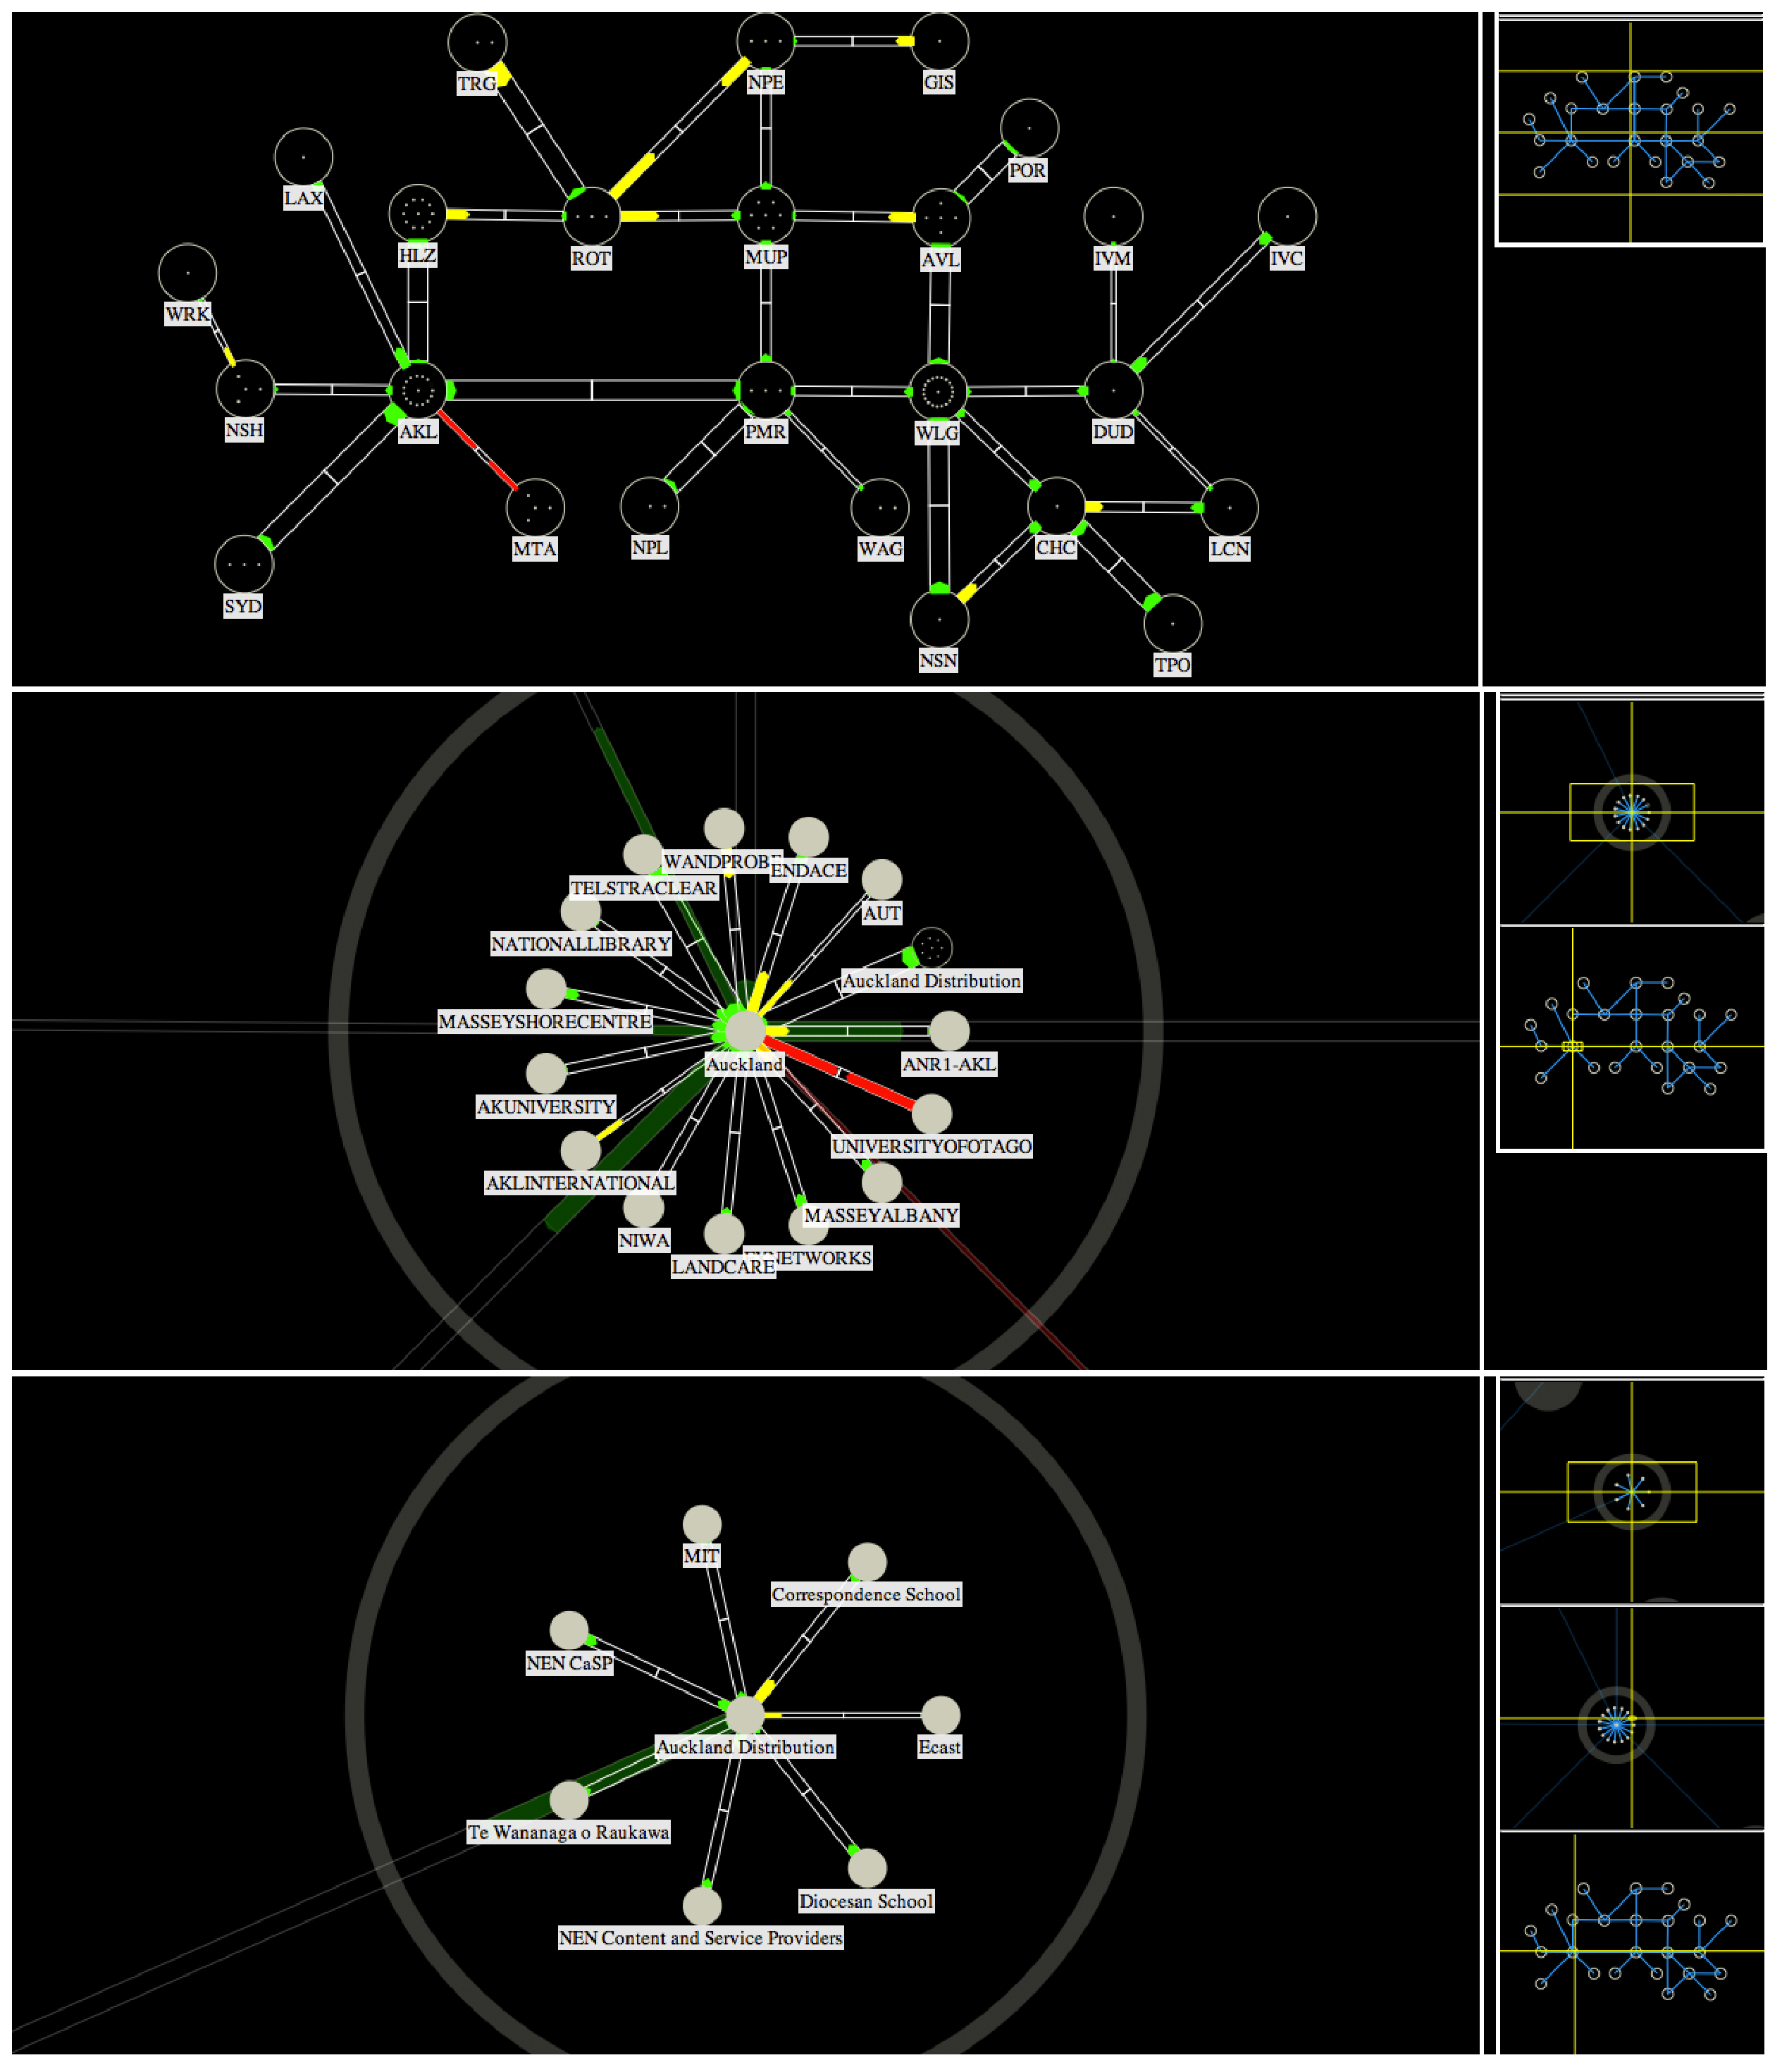
\includegraphics[width=170mm,height=197.95mm]{assets/overviews1-0.eps}
\caption{Three stacked screen shots of the KAREN map, each at different levels
of zoom. At deeper levels, more overviews are shown to be added to the stack
and the view port boxes change size and position accordingly.}
\label{fig:overviews1.0}
\end{figure}

\newpage

\section{Implementation} 
\label{sec:implementation}
  % Overall implementation
  % Client side / server side
  %   * Polling performance data
  %   * Interact with user to request more server side data
  %   * Or just change visualisation parameters

Details of the implementation of NetMapJs are described in this section. An
overview of how the tool works overall is given in Section
\ref{sec:client-server-model.impl}. The rest of the sections describe how
aspects of the visual design were implemented. Supporting functions such as
overlays and an editor are discussed in sections \ref{sec:overlays.impl} and
\ref{sec:editor.impl} respectively.

\subsection{Client / Server Model}
\label{sec:client-server-model.impl}
  % Give diagram of the over all structure of application
  %   * How the client side works in a lot of detail
  %   * How the Server side works in a lot of detail
  %       > Also state how much of server side was implemented
  %       > Not big focus of this project as specific to network

NetMapJs was implemented to run mostly on the client side with only some of the
work done on the server side. Figure \ref{fig:implementation-overview} shows the
main components of both the client and server side, and how they interact to
produce the final application. The NetMapJs application, shown in the client
side, is loaded from the server and then run in the client web browser. Initial
map layout data is then requested, visualisation data structures and events are
initialised, and a display is generated for the user. At this point the user has
full control to explore the visualisation.

The underlying network topology, performance values or other data may change
over time. For example, bandwidth data for links is likely to change frequently
throughout the course of a day. NetMapJs uses a data poller which is built using
JavaScript intervals that periodically and asynchronously polls for updated data
from the server side. This is done using AJAX methods to ensure that the
visualisation remains responsive and can be updated without refreshing the
browser page \cite{Paulson_2005}.

NetMapJs allows features of the maps to be manually adjusted, such as the node
positions. In a purely client side JavaScript application, user state is lost
when the web page is refreshed. To be able to make manual adjustments that can
be saved and reloaded, there must be a server side function with privileges to
read and write files to disk. When map configuration is saved, the NetMapJs JSON
data structures are passed to a state storage utility. This utility handles the
asynchronous transmission of the JSON data to the server. On the other hand,
when configuration needs to be retrieved, the storage utility requests the JSON
file from the server and proceeds to pass it back to NetMapJs where it will used
to rebuild the network map.

In this project, the main focus was on designing and producing the NetMapJs
client application. Only parts of the server side were implemented in order to
create a working application. The server side in Figure
\ref{fig:implementation-overview} shows how the components would fit together if
implemented completely. A web abstract programming interface (API) separates the
client and server functions to allow for visualisation design freedom that is
independent of web service constraints \cite{Wood_2008}. It also means that the
client is dependent on the API calls rather than any given server implementation.

The server side application handles saving and loading stored network map states
as well as gathering raw networking data through interactions with an adapter.
Adapters know about a specific networking data format such as RRD and how to
transform this into the generic JSON format that NetMapJs understands. As an
example, an adapter was developed for Rural Link that took their device
configuration file and produced a valid JSON structure that can be read and
visualised on the client side. The state and networking data is passed to the
client through the use of the web API.

\begin{figure}
\centering
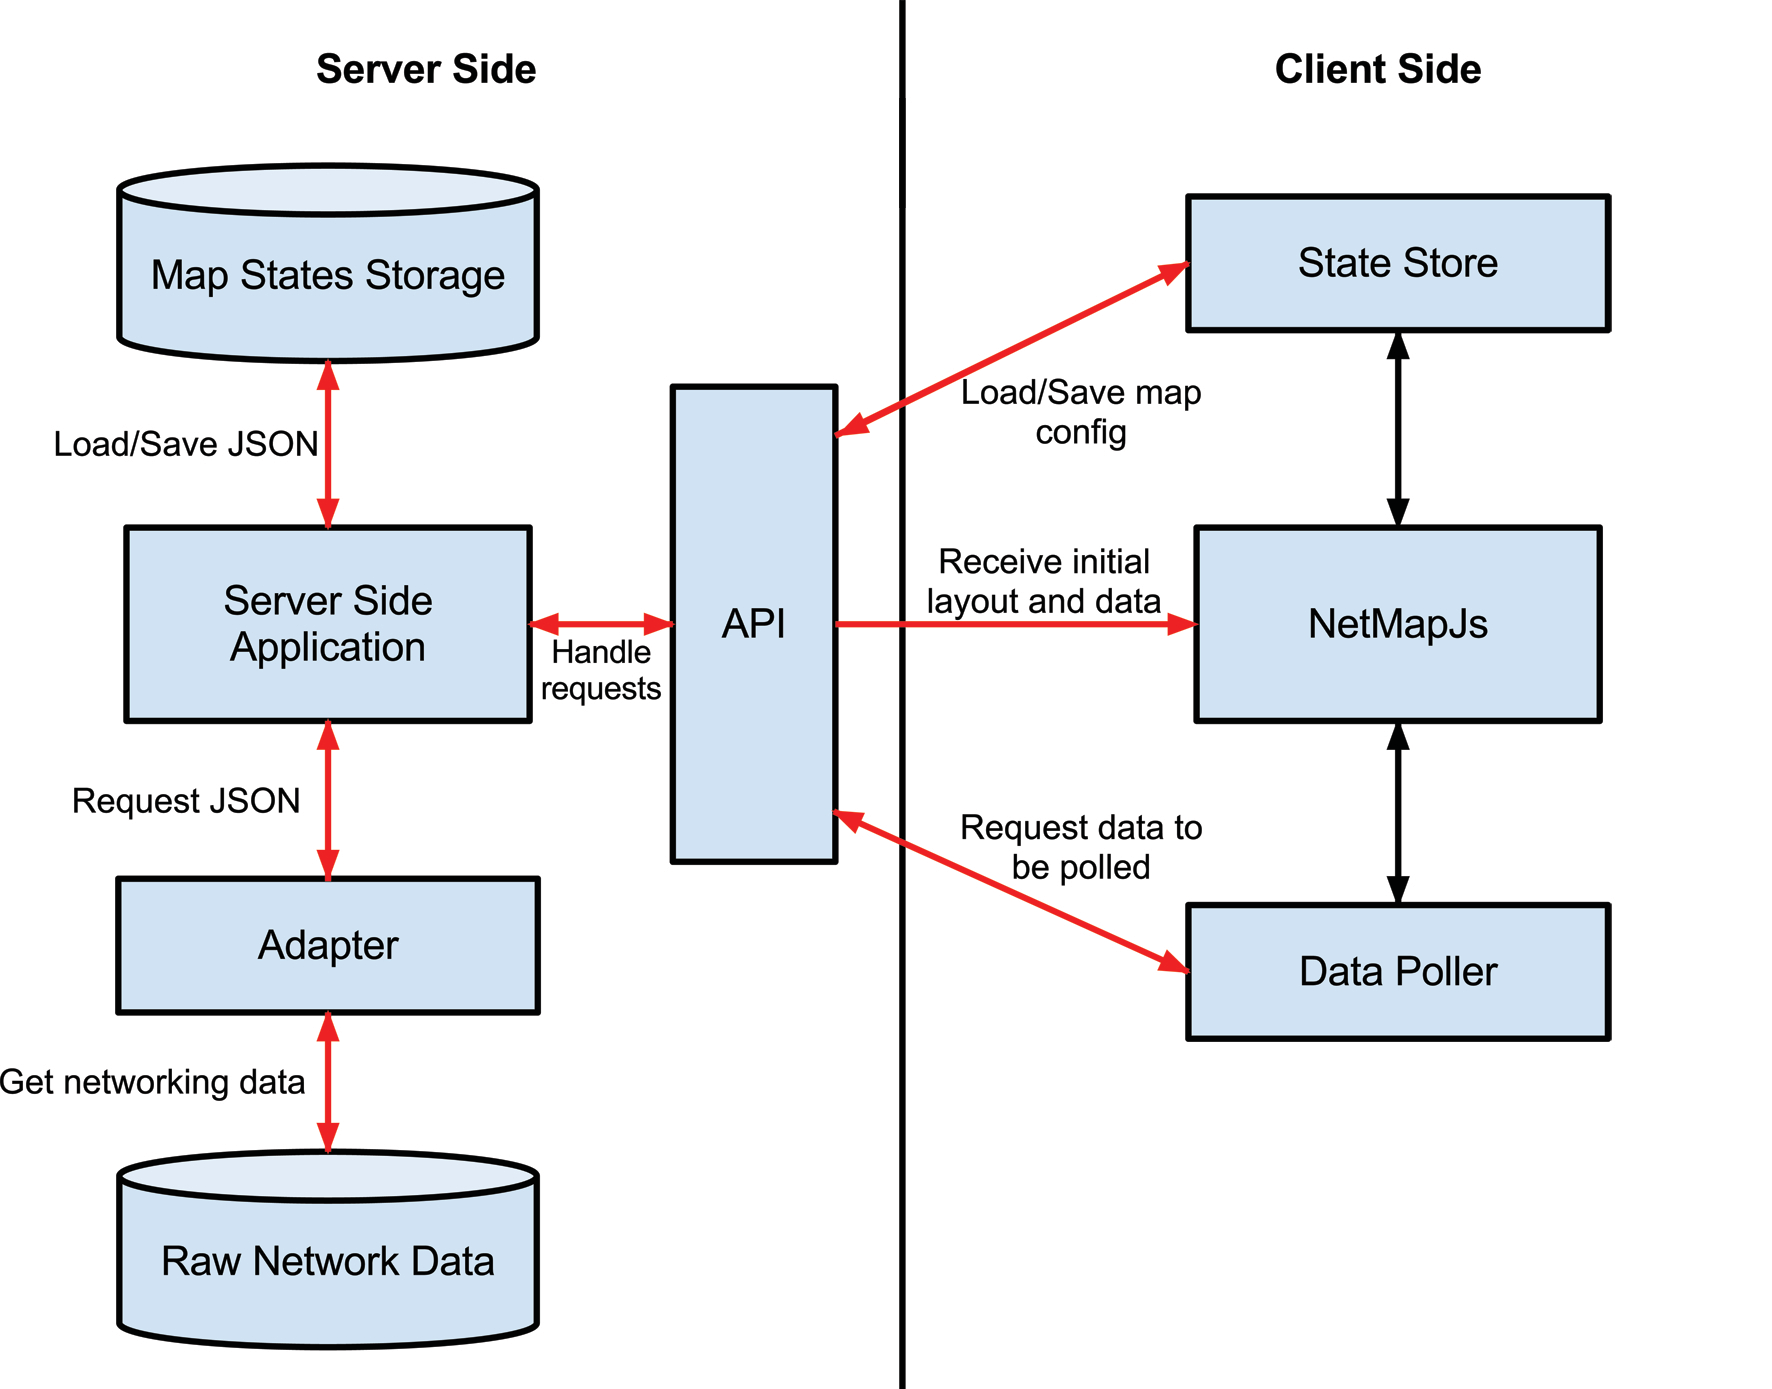
\includegraphics[width=170mm,height=133.26mm]{assets/implementation-overview.pdf}
\caption{Overview of the client to server side architecture.}
\label{fig:implementation-overview}
\end{figure}

\subsection{Nodes and Edges}
\label{sec:nodes-and-edges.impl}
  % How were nodes and edges implemented
  %   * Both have display method and contains method
  %   * Display: ..., Contains: ...
  %     > Dispay AND contains needs to scale in proportion with zoom
  %     > How did I do this?
  %   * People producing a view may implement their own functions
  %   * Pipe-edges are one of these.
  %     > How did I implement these
  %     > Look at edge data structures
  %     > rotated rectangular pipes, broken up into two sections
  %     > with height proportional to total bandwidth, length ...

The JavaScript InfoVis Toolkit has a built in system for handling the drawing of
nodes and edges. They each have a set of helpers which are objects that include
a display and contains method. The display method describes how a node or edge
should be drawn to the canvas and is called each time the map needs to be
redrawn. The contains method decides whether or not a point lies within the
bounds of the graphic once drawn onto the canvas. This is used as part of the
event system which loops over all contains methods to find a node or edge that a
user is interacting with. The helpers interface allows new edges and node types
to be easily implemented.

NetMapJs implements several different node and edge types to cater for various
functions. In particular, group nodes need to visually contain sub nodes and
edges need to consider the current level of zoom. As the user zooms into the
network map, edge widths are scaled in proportion such that they always remain
the same. This is required because in NetMapJs, quantitative variables may be
encoded by the edge widths. If the scale for the widths changed as the user
zoomed in, it would be difficult maintain an understanding of quantity. As more
edges are added at greater zoom levels, multiple scales would have to coexist
which would cause more confusion.

The main edge type that was implemented for NetMapJs was the bidirectional
divided pipe as described in Section \ref{sec:edges.vis}. Figure
\ref{fig:nodesedges1.0} shows how the edges are built using bandwidth as an
example. A rectangle is drawn between two nodes with arrows facing in both
directions. Sizes are calculated as shown, the canvas is rotated around a
central pivot point and then the final pipe is drawn.

The height of the rectangle is calculated by normalising the capacity and
factoring in the user defined line width and current scale offset.
Capacity is the total bandwidth available over the link and the normaliser is a
value that reduces the capacity value down to a smaller scale. The length of the
arrows are calculated as the proportion of the bandwidth over the total capacity
multiplied by the half of the rectangle's length.

% TODO: talk about label issues
% Canvas labels vs Div Labels relative to scaling

%\begin{verbatim}
%Metrics = {
%   bandwidth:   number,
%   capacity:    number,
%   latency:     number,
%   ...
%}
%\end{verbatim}

\begin{figure}
\centering
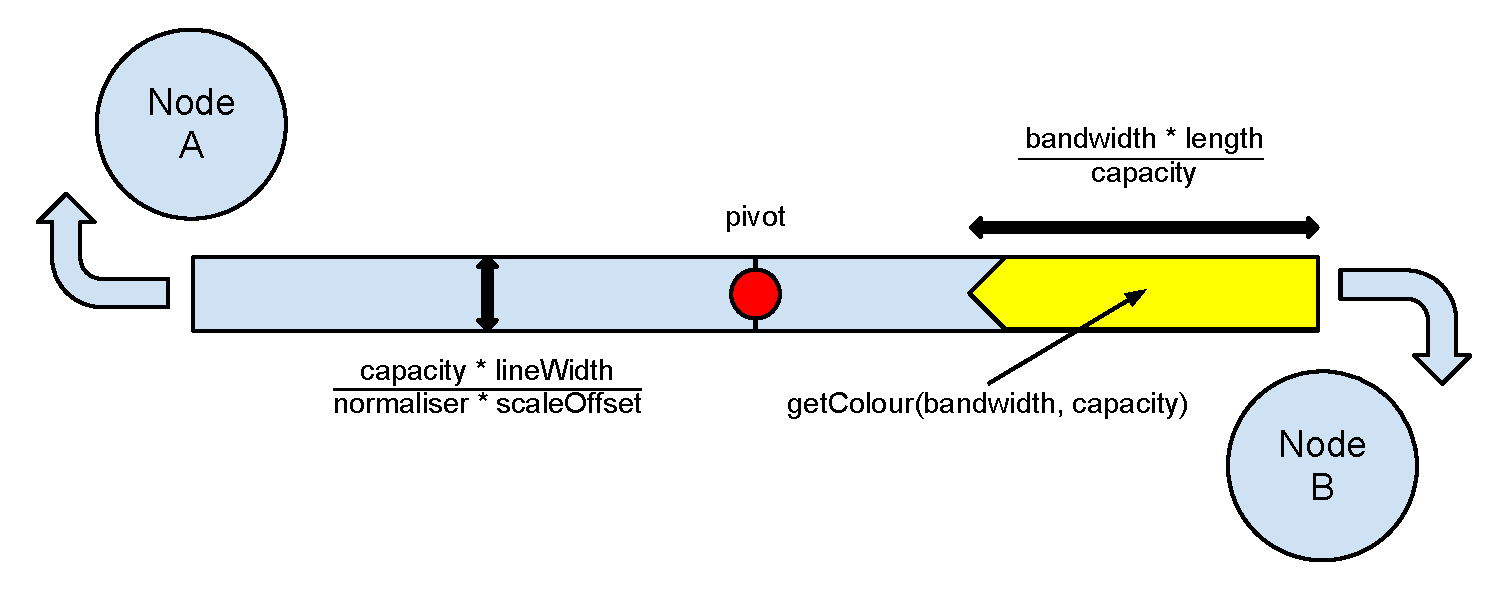
\includegraphics[width=170mm,height=63.24mm]{assets/nodesedges1-0.pdf}
\caption{A diagram showing how map edges that include bandwidth data are implemented.}
\label{fig:nodesedges1.0}
\end{figure}

% image nodes

\subsection{Groups}
\label{sec:groups.impl}
  % How were groups implemented?
  %   * Nodes can have parents
  %   * Parent nodes are group nodes
  %   * All the nodes that have a group node as a parent become its children
  %   * Functions
  %       > BuildGroups
  %           - Recursively build groups from top down
  %           - Extract all nodes that belong to the top group
  %           - On reduced set of nodes, extract all nodes that belong there
  %       > ComputeLayouts
  %           - Set the root of group if given (some layouts may use this)
  %           - Apply layouts to each group

Nodes can be assigned to a parent. If a node does not have a parent then it is
considered to be one of the top level nodes. The top level is the highest level
of the network map and is the starting point for grouping and depth algorithms.
All of the nodes that do have a parent, become part of a group.  Three methods
handle the group functionality: BuildGroups, ComputeDimensions and
ComputeLayouts.

BuildGroups recursively builds groups by assigning nodes and a depth level to a
parent. A depth level is the distance, in groups, from the top to the parent's
level. The function starts with the top level set of nodes and reduces it until
all of the nodes have been assigned a group and depth level. The
ComputeDimensions function loops through all of the groups and adjusts the node
edge sizes. Node dimensions are scaled by a factor of the node's group depth
such that deeper nodes appear smaller. Edges are assigned the line width of the 
parent which scales according to the current zoom level.

Groups can be assigned different layout algorithms for distributing nodes. The
ComputeLayouts function first sets the root of a group if this has been
specified in the initial JSON configuration. This is useful for algorithms that
require a root to be specified such as the star layout described in Section
\ref{sec:layouts.impl}. ComputeLayouts then loops through all of the groups and
applies the specified layout algorithm to the group or the default if none has
been chosen. 


\subsection{Layouts}
\label{sec:layouts.impl}
  % Overview of layout system
  %   How it is designed to be extendible
  %     > Implement generic interface
  %         - What does the Layout interface look like?
  %         - Methods etc, how they provide generic way - separating from data
  %         - Only know about node positions
  %     > Assign layout to group node
  %     > Allow to be changed at run time
  %
  % What layouts have I implemented?
  %   > Static (I did), Star (I did), ForceDirected (Arbor)
  %     - static - takes node ids mapping to x,y coordinates and loads them in
  %   > Basic overview of star layout (because I implemented it myself)
  %     - maybe include pseudo code for it
  %   > ForceDirected
  %     - describe how Arbor is integrated easily using a Layout implementation
  %

Nodes need a way of being positioned on the screen. In computer networks there
are many different layout styles that may make sense. For this reason, the
layout system was designed to be easy to extend. Layout algorithms take an
input, which is usually just a set of nodes and adjacencies, and output a set of
positions for each node. NetMapJs defines a layout interface as an object that
has initialise and compute methods. The layout is first initialised to set up
any initial parameters and then the compute method is called to calculate node
positions whenever they are required. The compute method may be called multiple
times for algorithms that change over time such as the force directed layout.
This system allows layout types to be changed at run time which could be used to
give the user the ability to switch algorithms to achieve a different view.

NetMapJs currently has three layout types implemented: static, star and force
directed. The static layout takes a set of node IDs that map to x and y
coordinates and loads them into the nodes objects. The positions are sourced
from the server that is keeping the state. The editor which is presented in
Section \ref{sec:editor.impl} can be used to create these static coordinates and
save them to the server.

The star layout algorithm places a given root node into the center of the screen
and then places the rest of the nodes, evenly spaced, around the circumference
of an invisible circle centered on the root. The radius of the circle is a
specified fraction of the parent group's width. This layout is limited by the
amount of space it uses due to the circular positioning of nodes. The space
between the center of the circle and the circumference where all the nodes are
located only used for edges. Also, the space between the circle circumference
and the parent node's bounds is completely unused. If the parent node was not
shaped like a circle then there would be gaps at the corners where the
circumference can not reach. It is also only appropriate to use when the
underlying network structure is star like.

The final layout algorithm, force directed, uses the Arbor library for
maintaining the node positions. The purpose of force directed algorithms is to
position nodes such that edges are similar lengths and there are as few
crossings as possible.  The initialise method of the layout interface creates
the particle system and the compute method transfers the positions from Arbor to
the node objects. This way, the compute method can be continuously called in
order to give an animated effect as the nodes move toward their ideal positions.

\subsection{Navigation}
\label{sec:navigation.impl}
  % How is navigation implemented overall:
  %   > Canvas translate/scale offset methods
  %   > At user defined level of scale, depth variable changes
  %   > nodes/edges that have depths less or equal to are shown. Others hidden
  %   > Mention labels
  %   > nodes/edges that have depth less than are drawn with lower alpha.
  %   > RenderFactory takes care of what to draw and what not to draw + alpha
  %   
  %   > Nav also effects edges with diff src and dst types
  %   > If edge connects an inner group node to another group with a lower
  %   depth...
  %
  %
  % Follow edges, zoom/center nodes
  %   > how are these implemented?
  %   > Follow edges:
  %     * For a given edge that the user has hovered over
  %     * Are both nodes in the canvas bounds - then do nothing if clicked
  %     * Are no nodes in the canvas bound - then do nothing if clicked
  %     * If one node is visible on the screen then set the other node as dest
  %     * Follow linear path towards dest node until it is in screen centre
  %
  %   > zoom / center nodes
  %     * If user clicks on a single node
  %     * calculate translation difference to center it
  %     * calculate scale difference to zoom in on it
  %     * Set an interval that performs small interations to produce animated
  %     look
  %
  % Pan and Zoom + Space Scale diagrams - Space–scale Diagrams:Understanding Multiscale Interfaces
  % Pans are linear, zoom is logarithmic

Navigation is implemented through the use of the Canvas translate and scale
offset functions. The scale offset function performs a geometric zoom on the
canvas which allows for full space-scale navigation in 2D \cite{Furnas_1995}. In
order to achieve semantic zooming where the information content changes based on
the scaling, components on the network map must be matched to the levels of
zoom. In NetMapJs, when a view is created it is assigned a set of scale offsets
which define the points where information content should change. These offsets
are computed with the depths of nodes to determine when they should be displayed
as shown in Figure \ref{fig:nav2.0}. Group nodes are automatically assigned a
depth based on the number of parent nodes between them and the top level.
Manual assignment of depth values is also possible. 

A rendering function handles when and how each visualisation aspect should be
displayed. Nodes, labels and edges that have a depth value that is less than or
equal to the zoom offset are visible in the map. Nodes and edges that just have
a depth less than the offset are drawn with a lower alpha value. This creates
the desired effect of fading out nodes above the current level. Edges have an
additional condition that handles the case when edges join nodes of different
groups. Those edges that extend from one group to another deeper group's node
should only be partially displayed. That is, the edge should start from the
displayed node and extend only to the edge of the group that contains the deeper
node.

As described in Section \ref{sec:navigation.vis}, there are two navigation
support features to assist the user in moving around the network map. The follow
edges feature allows the user to click on an edge to be transported to the node
on the other end. This is implemented by following a set of conditions. For a
given edge that the user has clicked on, if both or none of the source and
destination nodes are within the visual map space, then do nothing. If, however,
one of the nodes is in the visual space then this becomes the source and the
destination node is on the other end of the edge. The view port then follows a
linear path towards the destination by translating the canvas until the node is
centered on the screen. The zoom and center feature allows the view port to
quickly focus on a node. This was implemented by calculating the translation
difference required for centering and the scale offset necessary to zoom in on
the node. A JavaScript interval is set to animate the view port into the new
position by incrementing coordinates in each step.

\begin{figure} \centering
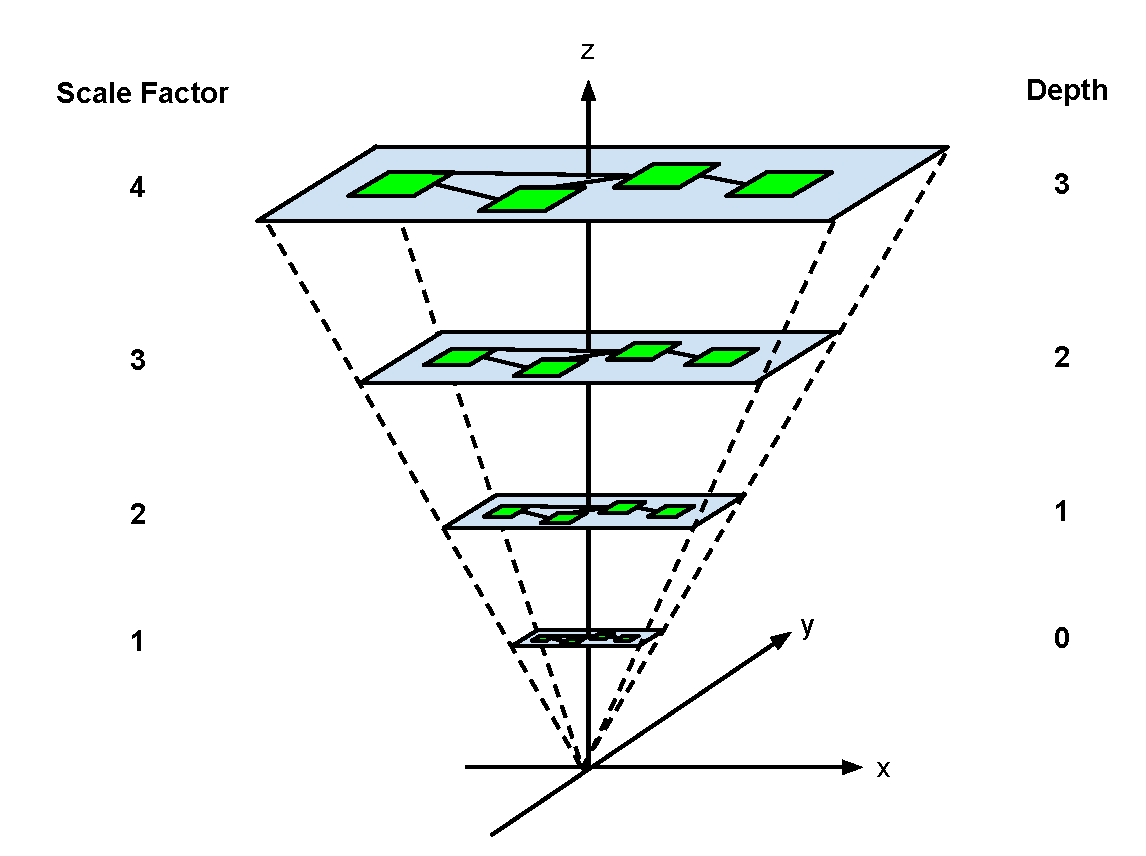
\includegraphics[width=120mm,height=87.2mm]{assets/nav2-0.pdf}
\caption{A space-scale diagram showing different levels of magnification being
mapped to depth levels where the detail changes. (Adapted from Furnas and
Bederson \cite{Furnas_1995}.) } 
\label{fig:nav2.0} 
\end{figure}

\subsection{Overviews}
\label{sec:overviews.impl}
  % How are overviews implemented?
  %
  %   > Based on scale offsets - add/remove more overviews
  %   > Two classes - overview manager and overview.
  %   > Instances of an actual network map
  %   > Draw crosshair and view port box over top of it
  %   > Update this by listening to plot redraw events fired by the main map
  %   

Overviews help the user to maintain overall context as they zoom and move around
the network map. At higher levels of zoom, additional overviews are required to
show each depth level of the network. An overview manager class handles the
adding and removing of overviews when the main network map is navigated. An
overview consists of a DOM container, a minimalistic network map instance and set
of functions that handle the interaction with the main view. Overviews are added
when the current depth level of the network map increases and removed when it
decreases. The depth level is defined by the current level of zoom compared with
the user defined scale offset values.

Overviews require a two way interaction with the main network map instance. If
the user clicks on the overview to move the view port box to another position,
then the main map needs to be translated accordingly. This translation
difference is calculated by converting the overview coordinates of the mouse
click into the main network maps geometric space and then subtracting the two.
When the user navigates in the main view, the overview view port boxes need to
move to reflect the change. Overviews listen for the redraw event to be fired by
the main network map. When the event is triggered, the overview calculates new
coordinates and dimensions for the view port box, and then redraws it.


\subsection{Overlays}
\label{sec:overlays.impl}
  % Similar to overviews in that there is an overlay manager and overlays
  % 
  % Overlays contain an update method which is passed:
  %   > The visualisation object, graph object and the canvas
  % Overlays can be started and stopped and redrawn
  %
  % The overlay manager attached to a visualisation object
  % Overlays are drawn onto its canvas
  % The manager listens to redraw events
  %   > and refreshes the overlay instances when necessary. 
  % 
  % TODO: add overlay screenshot here

Overlays provide a way of adding additional visual features on top of the
network map after it has been drawn. An overlay instance contains an update
method that is called each time the overlay needs to be drawn. The method is
passed a reference to the main visualisation object, the node and edge graph
structure and the HTML canvas. These three references give the update method
access to enough data to render overlays positioned relative to the network map
elements. Overlays also contain methods to be started, stopped and redrawn.

A manager class is used to keep track of all of the overlays. It is assigned a
network map object and uses it to pass the appropriate parameters to the overlay
update methods. Overlay objects may be added or removed from the manager.
Network map redraw events are bound in the same way as overviews. When this
event is fired, the manager loops through all of its overlays and calls their
update method. 

One of the uses for the overlay functionality that was identified early in the
project and later requested for the KAREN map, is the displaying of virtual
local area networks (VLANs). Different VLANs may take separate paths through a
given network and may have their own set of performance metrics. An overlay that
visualises VLAN flows separately for the KAREN network is shown in Figure
\ref{fig:overlays1.0}. The purple lines shows the edges that the VLAN is
attached to. Zooming into the map further would show the connections within sub
groups. VLANs can be changed or turned off using the drop down box on the right
hand side on the display.

\begin{figure} 
\centering
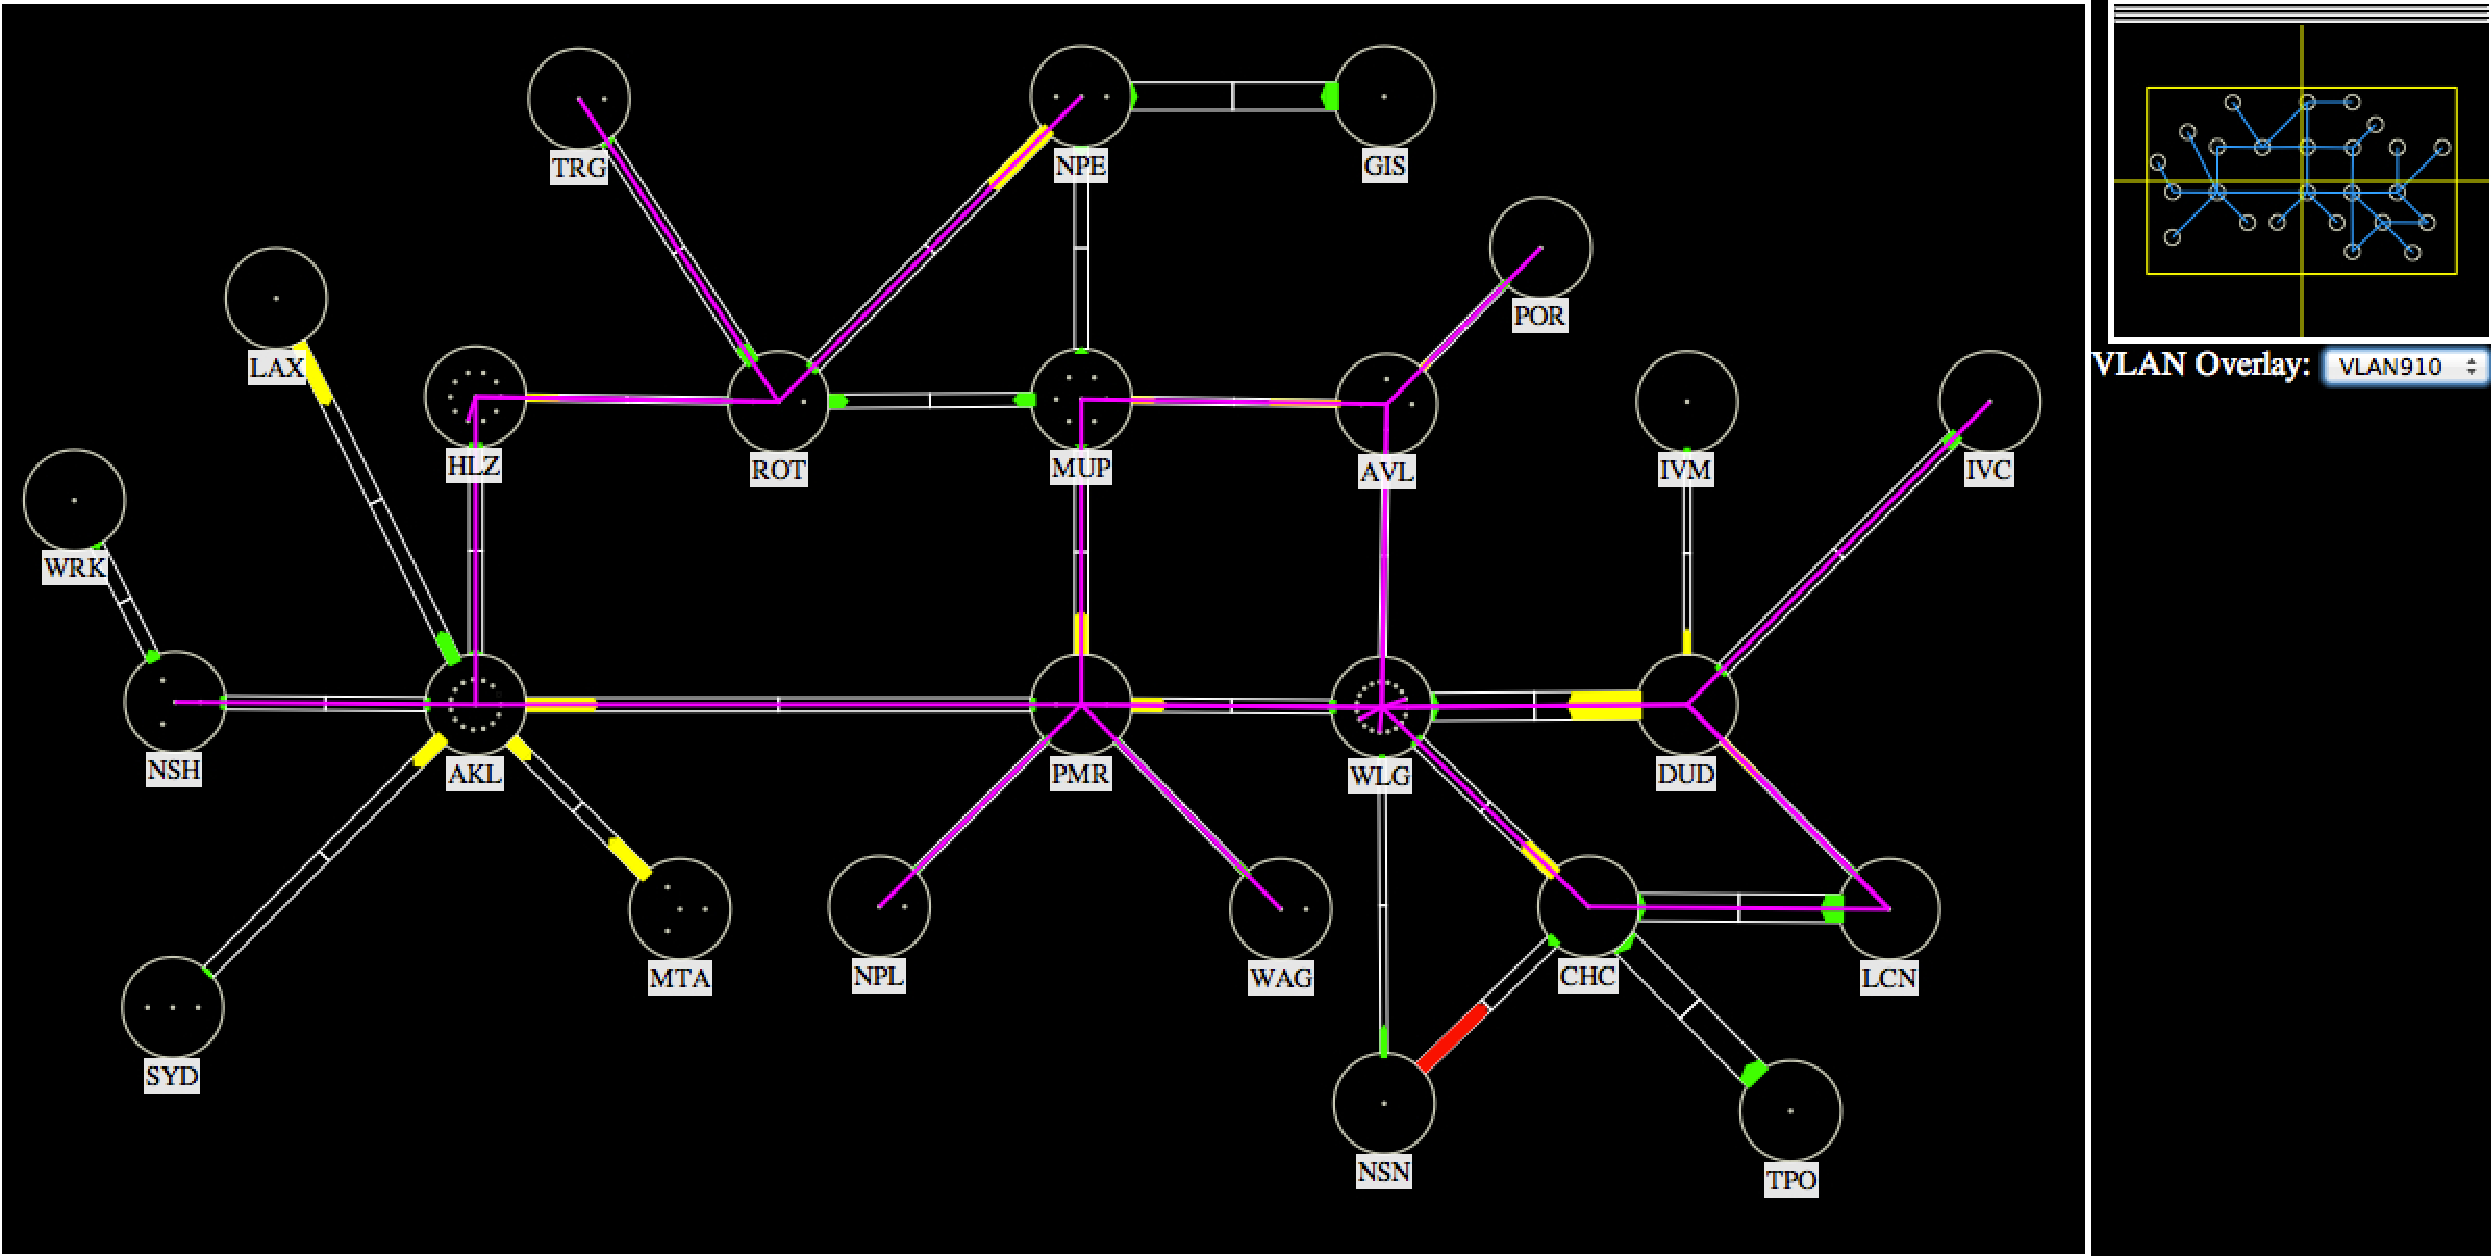
\includegraphics[width=170mm,height=85.71mm]{assets/overlays1-0.pdf}
\caption{VLAN 910 for the KAREN network visualised using the overlay
functionality.}
\label{fig:overlays1.0} 
\end{figure}

\subsection{Editor}
\label{sec:editor.impl}
  % Overview of the editor
  %   Why do we need it?
  %     - touch up positions, apply layout algorithms, set nodes parameters
  %     - Save/load
  %   How does it work?
  %     - Built using HTML, CSS, + a special network map view
  %     - View allows moving nodes and should allow applying parameters etc
  %     - Saving / Loading. JSON. Then loaded by a main map view
  %   How far did I get with it?
  %     - Ideally integrate layout algorithms with manual positioning for more
  %    control 
  %   

A visual editor that allows map views to be defined in real time is particularly
useful for getting visualisation parameters right. Ideally the editor should be
able to perform minor alterations to node positions, apply layout algorithms to
groups and set node and edge parameters. For example, different layout
algorithms may need to be compared to find the best fit and some nodes may need
minor subsequent position adjustments. The view, including all of the set
configuration, needs to be able to be saved and loaded back later.

NetMapJs includes a basic editor that currently only supports nodes being moved
around a grid. More work is required to produce a complete editing system. The
editor was built using a combination of HTML, CSS, JavaScript and a special
network map view. The view is an instance of the NetMapJs visualisation class
that adds extra functionality to load and update node positions as they are
clicked and dragged. When the view needs to be saved, the JSON data is taken
from NetMapJs and sent to the server using AJAX. Previously saved views are
loaded by reversing this process.

The editor was used to make the KAREN network map which is shown in Figure
\ref{fig:editor1.0}. An image showing one possible map design was copied by
manually positioning nodes using the editor until a similar layout was achieved.
The editor figure shows grids being used effectively for accurate node
positioning and spacing. Zooming and panning functionality is also supported in
the editor.

\begin{figure}
\centering
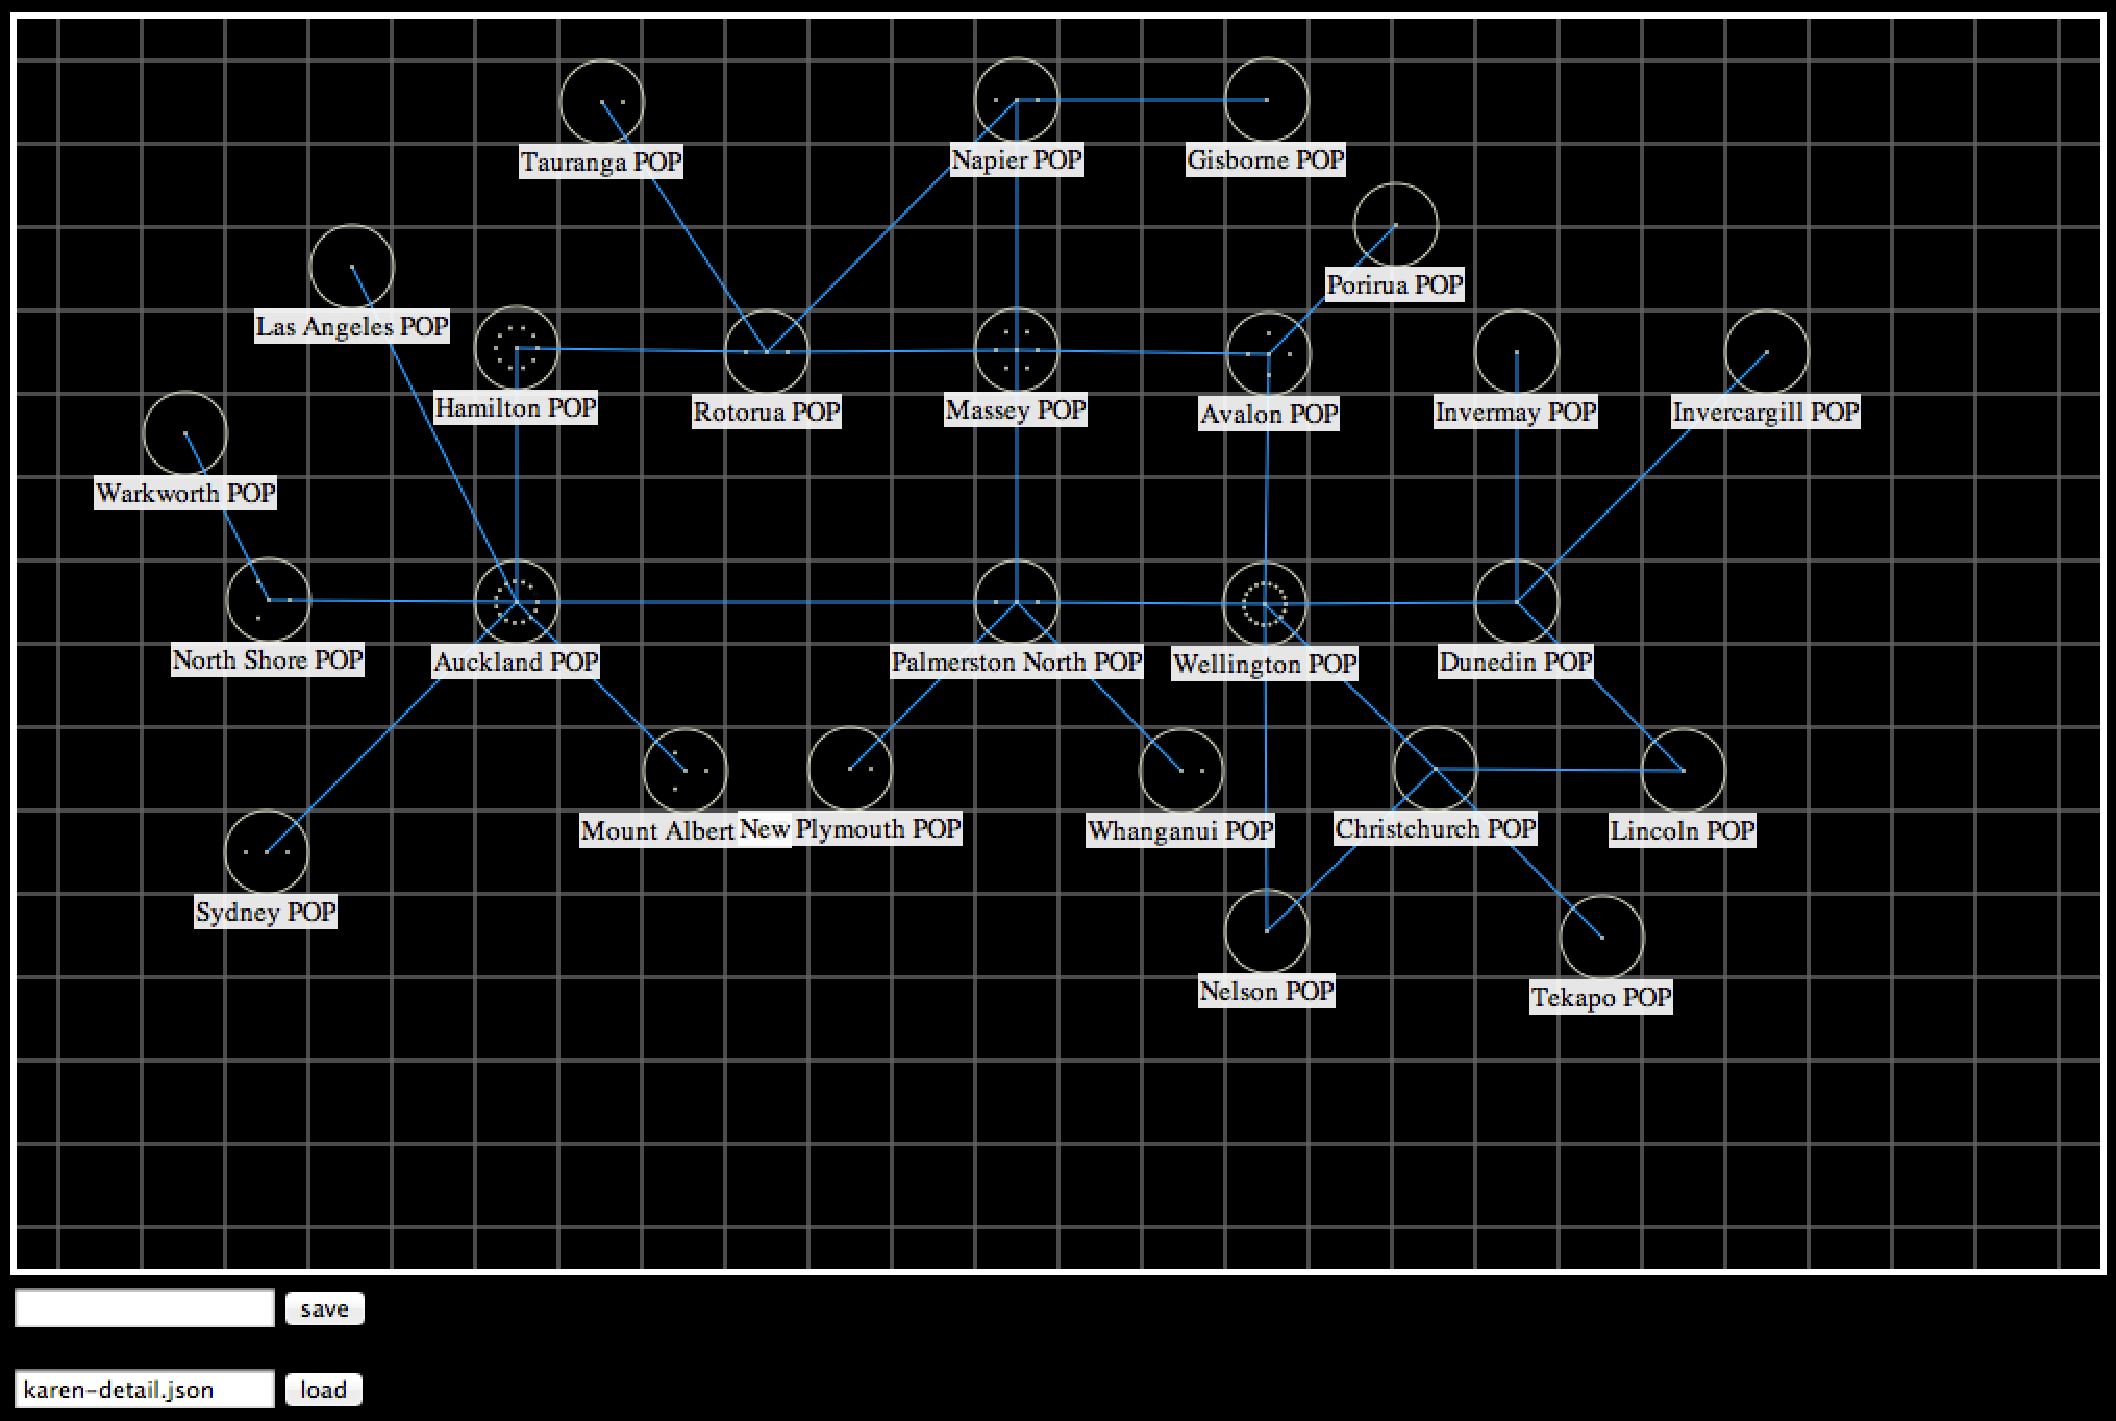
\includegraphics[width=170mm,height=120.16mm]{assets/editor1-0.pdf}
\caption{A screen shot of the KAREN network map loaded into the view editor.}
\label{fig:editor1.0}
\end{figure}

%TODO
%\subsection{Layers}
% how I tried and failed (Network descriptor language) how somewhat allow for
% manual layering
% Maybe just add a Problems Faced section?? - No add Discussion section just
% before conclusion

%\subsection{Debugger}
%\label{sec:debugger.impl}

\newpage

%\section{Deployment Examples}
%\label{sec:deployment-examples}

\section{Evaluation}
\label{sec:evaluation}
  %
  % How was the evaluation conducted:
  %   > send designs along with some evaluations questions
  %
  % KAREN
  %   > Strengths
  %     * VLAN traffic can be viewed separately
  %     * At high level, can see what PoPs have the most connected sites
  %     * Pipe widths are good
  %   > Weaknesses
  %     * Zooming should have limits
  %     * Some design choices such as fonts make label readability hard and
  %     colours such as red on black
  %     * Zooming - should be based off mouse position not screen center
  %     * Want to be able to resize the window
  %   > Comparison to PHP network weathermap
  %     * Once some the discussed weaknesses ironed out, will make a nice
  %     looking upgrade.
  %   > Would they consider using it
  %     * Yes.
  %     * Zoom functionality and ability to view VLANs separately
  %     * But need to be able have KAREN branding with colours and fonts
  %   > Any other feedback
  %     * Nice looking start
  %     * provoked thought within the KAREN team.
  %
  % Same for Rural Link
  %

An evaluation with network engineers from Rural Link and KAREN was performed to
analyse the strengths and weaknesses of NetMapJs. The redesigns of their network
maps were sent along with a set of questions to people in the respective
networks.

\subsection{KAREN}

KAREN liked that, at a high level of the map, they could still see which PoPs
have the most connected sites due to distant nodes being shown in basic detail.
They found that the pipe edge widths were effective at showing differences in
bandwidth between nodes. Being able to view VLAN traffic separately was another
advantage. KAREN also identified weaknesses of the map. Zooming in and out
should have hard limits such that the user can not accidentally scale too far in
either direction. Some of the design choices such as font and colours also make
some parts of the map hard to see. 

When asked to compare NetMapJs to PHP Network Weathermap, KAREN stated that some
of the zoom functionality and the ability to view VLANs separately were the most
significant advantages over their current implementation. They reported that
once the discussed weaknesses were ironed out, NetMapJs would make a good upgrade
to their current tool and they would consider using NetMapJs as a replacement
network map. They noted that the ability to add specific branding aspects such as
colours and fonts would be required. Overall, they liked the look of the network
map and mentioned that it has provoked some thought within the KAREN team.

  % Strengths 
  %   > Also think dynamic sizes for links and nodes could be really interesting
  % given live data.
  %   > Navigation combined with the overview plots produce really good
  % interactivity.
  %   > Sub groups work well at hiding structure
  %   > VLAN very good 
  %
  % Weaknesses 
  %   > Just looking nicer - UI around sub groups could be improved, more visual
  %   hints for moving between sub groups.
  %   > Manual layout is often still great to get a good, useful map. Multiple
  %   selectable layout nodes could allow you to switch between defined
  %   layouts. Eg geographical, logical or automatic.
  %
  % Comparison to Nagios
  %   > Much more interactive. Even more so that than the new Icinga NMS (cite).
  %   > Nagios doesn't deal with loops, its layouts are not very stable
  %   > No integration of performance data at all.
  %
  % Would they consider using it?
  %   > Yes
  %   > Would need to see how live data looks using the link utilisation
  %   graphics.
  %   > Also UI needs to be polished - they use a big screen for their
  %   monitoring visualisations.
  %
  % Any other feedback?
  %

\subsection{Rural Link}

Rural Link commented that the dynamic sizes for links and nodes could be really
interesting given live networking data to view them with. They thought
navigation combined with the overview plots supported effective interactivity.
Viewing VLANs separately were also seen as a strength of NetMapJs. It was
suggested, like with KAREN, that the overall user interface needs some
improvement. For example, more visual hints for moving between sub groups along
the edges would make that feature more obvious. Rural Link suggested using
multiple, selectable layout types to allow the user to decide on the best
positioning. Geographic, logical and automatic are possible layouts types that
were suggested.

Rural Link was also asked to compare NetMapJs to their existing Nagios network
mapping tool. They found it to be much more interactive, even more so than the
new Icinga network management system \cite{Icinga_website}. Nagios does not deal
with loops, its layouts are not very stable and there is no integration of
performance data in the maps. They would consider using it as a replacement to
their current map provided that it is easy to import networking data and that
the user interface is suitably improved. This is particularly important because
a large screen is used in their office for viewing visualisations. 

\newpage

%\section{Future Work}
%\label{sec:future-work}
%\newpage

\section{Conclusions and Future Work}
\label{sec:conclusion}

  % What were my results? (Don't state here, but important to think about)
  %   * Network Map Implementation (HTML5)
  %   * Semantic zoom functionality
  %   * An extensible layout system
  %   * New edge design
  %   * The beginnings of an editor
  %   * An overlay system
  %   * Navigation support features such as interactive overviews
  %
  % Where the results can lead you?
  %   * NetMap implementation - incorporate as part of NMS
  %   * Semantic zoom could be investigated further such as loading only visible
  %   data at a time. Link to network layers somehow
  %   * Layout system - include many more layout algorithms, particularly those
  %   that are effective at displaying networks
  %   * 
  %
  % What are the next steps to take?
  %   * Incorporate graphs of metrics, triggered by events
  %
  %
  % What other questions do my results raise?
  %   * New node design - is there other, better ways doing it
  %   * 
  %
  % Discuss possible branches of future work
  %   > Incorporate the map as part of a network management system
  %   > Experiment with more layout algorithms
  %   > Look into the possibility of effectively incorporating layers
  %   > Generate adapters to take common network data types such as RRD

There are several possible paths to take for future work resulting from this
project. Semantic zoom could be investigated further to explore possible uses
with respect to network maps. Early on in this project, the ability to relate
different network layers together through the use of zoom was considered but
little progress made. Very large networks, such as an entire autonomous system,
may require that zooming splits up data requests and only displays currently
visible depth levels. 

This project only considered two automatic layout algorithms out of the many
that are found in literature \cite{Battista_1994}. Including more layout
algorithms, particularly those that are known to be effective for computer
network visualisation, would allow a more diverse set of networks to use the
tool. One notable feature included in some other network mapping tools is the
inclusion of graphs of relevant metrics. For example, graphs of bandwidth over
time are useful to help network engineers identify when anomalies occur.  These
graphs could be included as part of the visualisation itself through the use of
user interaction triggered events.

NetMapJs includes a rich design for displaying network metrics between two nodes
as part of the actual edge graphics. A survey of node and edge designs for
computer networks would support the development of further network map displays.
In this project, NetMapJs was developed as a stand alone application.
Incorporating the tool into a network management system such as
Nagios \cite{Nagios_website} or OpenNMS \cite{OpenNMS_website} would be a good
extension to allow NetMapJs to be used with a minimal installation and setup
overhead.

  % used web technologies such as Canvas and JavaScript (identified and used c).
  % used lots of libraries
  % scalability - network hierachies + semantic zooming
  % grouping - specific layouts and depth
  % overlays - a generic way of allowing developers to add additional drawings
  % overtop of the existing display.
  % overview - maintain sense of positioning in the overall network
  %
  % Results *
  % Actual implementation - NetMapJs
  % Real examples using real datasets
  % successful evaluation (they want to use it)


The goal of this project was to produce an improved computer network map
display. This was achieved by identifying weaknesses in existing implementations
and looking at ways of addressing them. A web based application called NetMapJs
was developed to generate and control interactive network map displays. The main
features of NetMapJs developed for this project are:

\begin{itemize}
  \item Data adapters that separate raw data from the actual visualisation
  \item Semantic zooming and panning combined with sub network hierarchy for
  improved scalability
  \item Automatic layout algorithms that can be applied to sub network groups
  \item Stacked overview boxes that help users maintain a sense of positioning
  as they navigate the map
  \item An overlay system that provides a generic way for developers to add in
  additional graphics over the network map
  \item An editor view that allows users to statically position nodes
\end{itemize}

Through the use of these features, NetMapJs was able to address some of the
limitations of existing network map implementations as described in Section
\ref{sec:introduction}. The outcomes of of this project in terms of network map
improvements are:

\begin{itemize}
  \item Rich user interactivity allowing the user a lot of control over the
  visualisation
  \item Scalable network map design that allows large networks to be displayed
  \item A web browser based display using HTML5 specification that doesn't
  require specialised software
  \item Informative edge graphics incorporated into edges that effectively show
  network metrics using sound information visualisation theory 
\end{itemize}

NetMapJs was tested using real topology data sourced from the Rural Link and
KAREN networks. An evaluation with these two networks was successful and pointed
out the strengths and weaknesses of NetMapJs. Engineers from both of the
networks indicated that this network map would be an improvement over their
current tool in use and that they would consider using it once the software was
polished and their concerns addressed. In particular, with an improved user
interface, a more complete set of layout algorithms and a completed
client/server side model implementation, NetMapJs will be ready for live
deployment in real world systems.

\newpage

%TODO
%\section{Acknowledgements}
%\label{Acknowlements}

\bibliographystyle{plain}
\bibliography{520-report}

\newpage

\appendix
\appendixpage

\section{KAREN PHP Network Weathermap}
\label{app:karenphp}
\centering
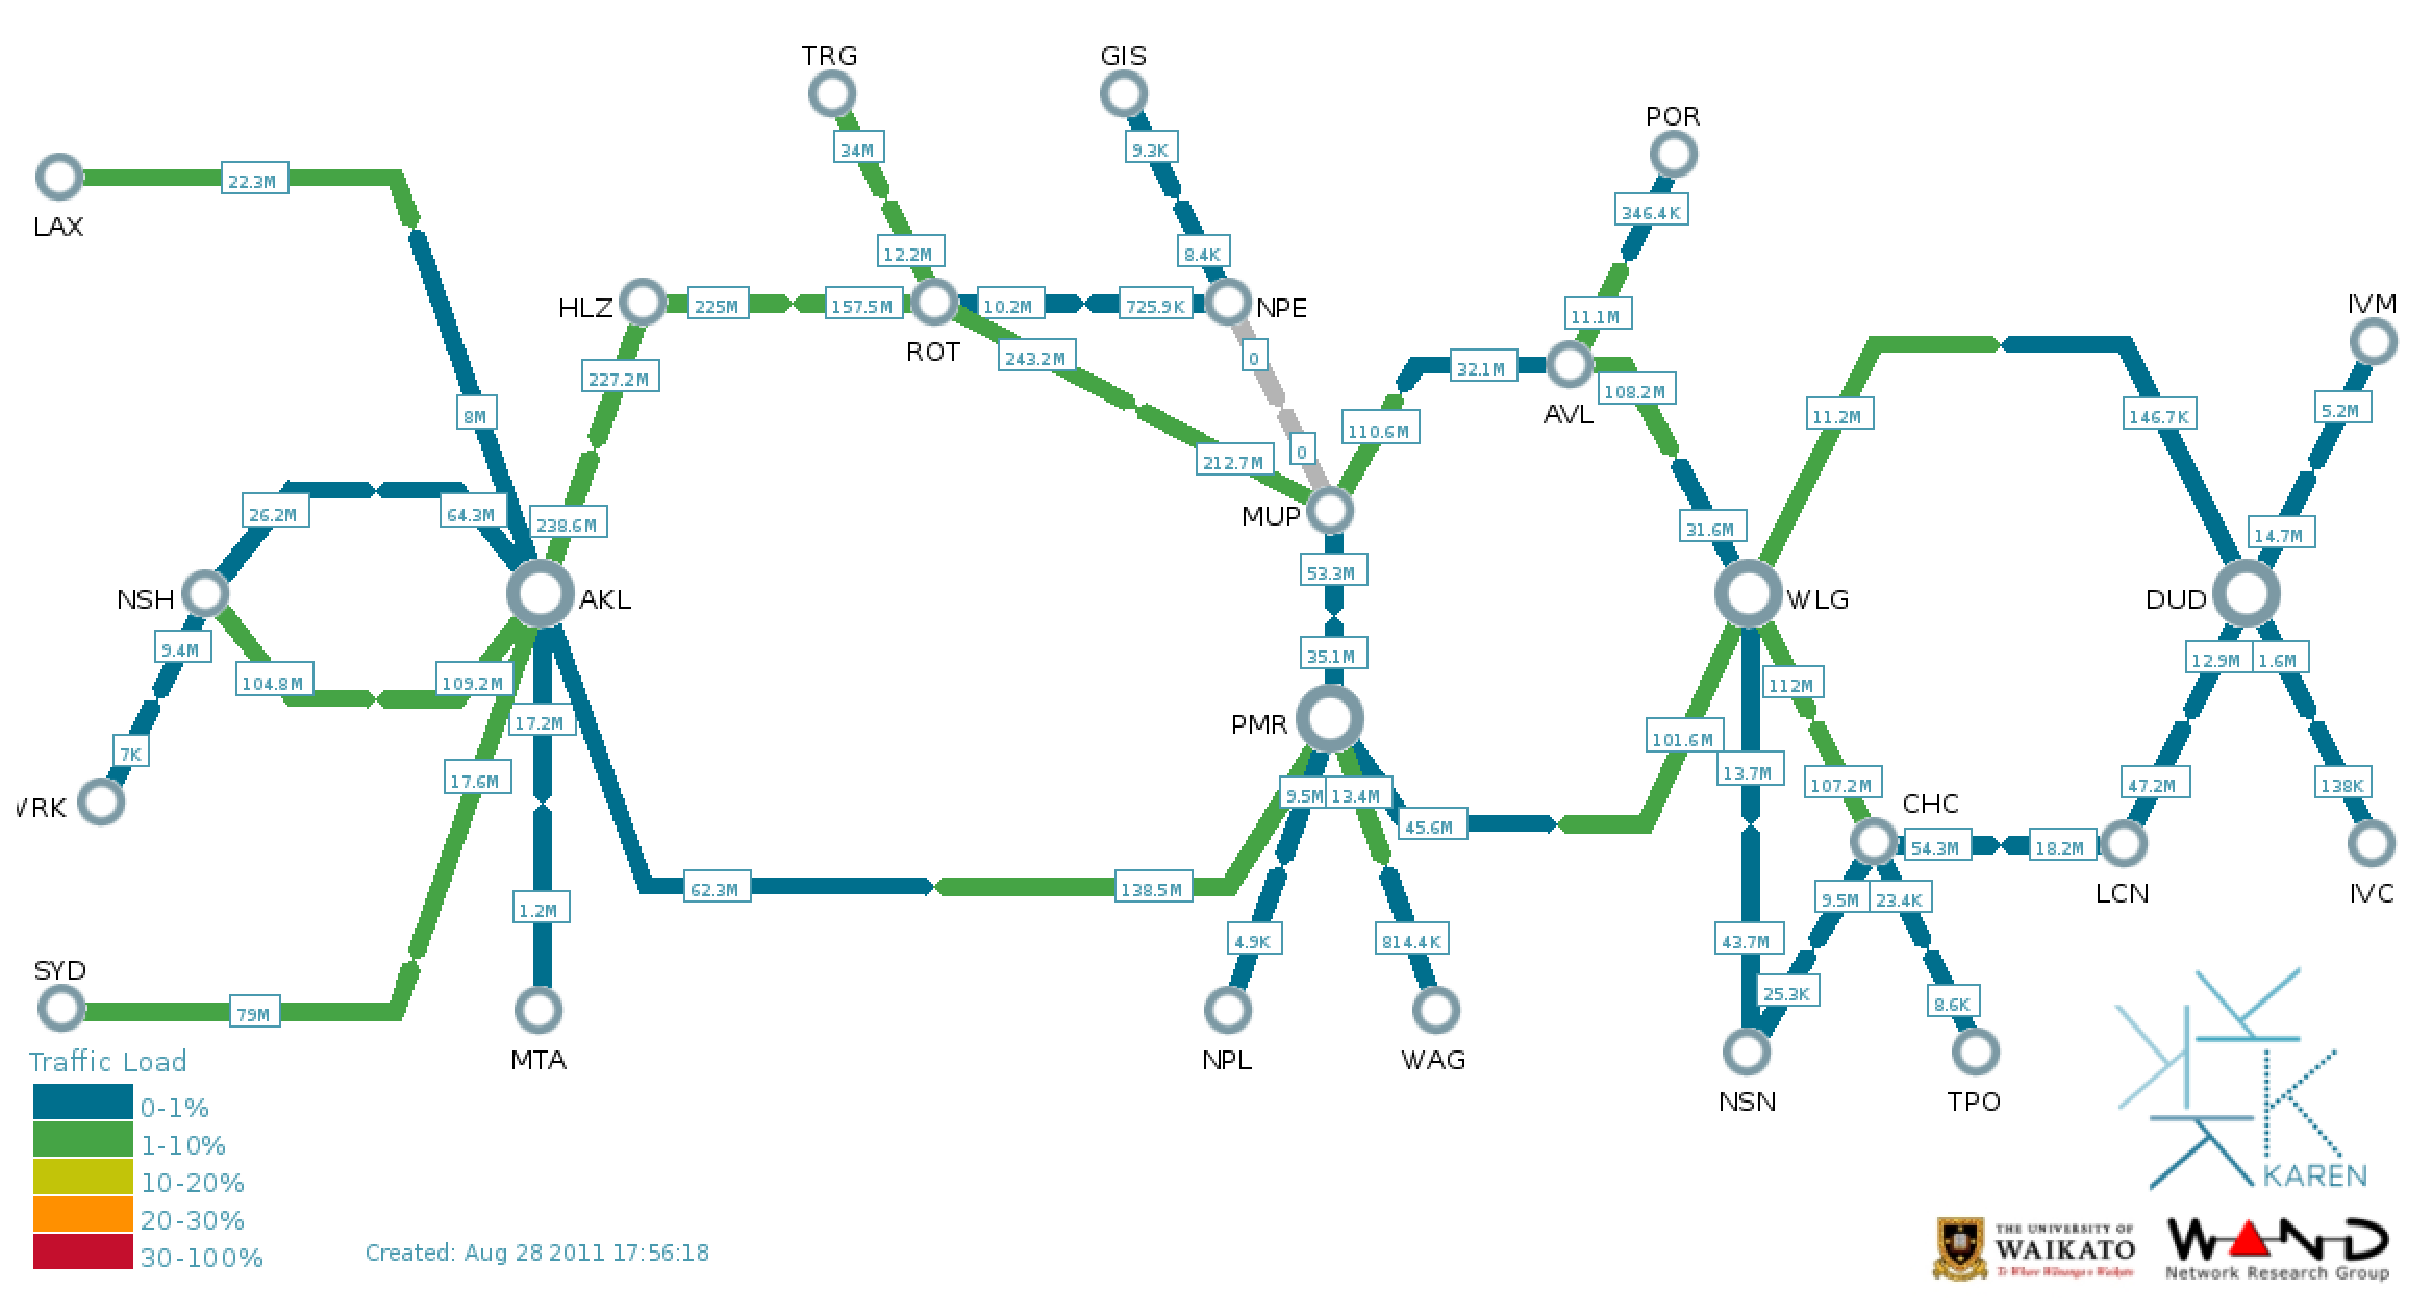
\includegraphics[width=170mm,height=90.76mm]{assets/karen-phpweathermap.eps}

\newpage

\section{Rural Link Nagios Network Map}
\label{app:crcnetnagios}
\centering
\includegraphics[width=170mm,height=136mm]{assets/rurallink-nagios.eps}

\newpage

\section{Evaluation Question Set}

\begin{enumerate}
\item What do you think are the strengths of NetMapJs?
\item What are the weaknesses of NetMapJs?
\item Would this map be one that you would consider using in your network? Why? / Why not?
\item How does NetMapJs compare with your current network map?
\item Do you have any other feedback?
\end{enumerate}

\end{document}
